\chapter{Results}
The three path planners (NHV, N-NHV, and MCPP) introduced in Chapter \ref{ch:pp} all aim to reduce the overall prediction uncertainty of a field given a limited amount of flight time. They accomplish the task by calculating variances of a target field's predictions and attempting to choose a trajectory that reduces overall uncertainty. 

The number of trajectories compared in both the NNHV and MCPP methods is $N=5$. For the MCPP method, an additional $M_{mc}=20$ Monte Carlo trajectories are calculated for each of the $N$ trajectories. The target field size of the fields compared in the simulation have unit-less vesicle dimensions of $100\times 100$. Two random number generator seeds ($2$, $3$) are used to generate two sets of runs in an effort to show the methods for a variety of random fields. The autocorrelation factors of the field will be varied in an effort to show the effectiveness of the methods for different field statistics. When the prediction variances of the methods are compared, the values are normalized to an a priori mean variance, which is equal to the mean variance of the field generated from running a Kriging prediction on the equivalent field from a set of five samples taken from the main diagonal vesicles of the target field.

\subsection{Prediction Error Calculation}
The quality of each path planner will be judged by its ability to explore a field in a fixed amount of time. The prediction error of each method will be used as a metric of path planning quality. The actual values of the fields scanned are known in simulation, and for each rerouting iteration, the predictions and prediction errors will be recalculated.

The prediction error function, erf$(Z,\hat{Z})$, will be the average root mean square (RMS) value for all $N$ field predictions made, point by point, on the actual field, $Z$, and the predicted field, $\hat{Z}$.

\begin{equation}
\text{erf}(Z, \hat{Z}) = \frac{1}{N}\sum_{\forall i \in Z} (Z(\vect{s}_i) - \hat{Z}(\vect{s}_i))^2
\end{equation}

\section{Comparing to Greedy Next-Best-View}
A course field of size $20 \times 20$ vesicles was generated with a autocorrelation factor, $\sigma_{field}$, equal to $4$, and limited to a $30\%$ scan.

\begin{figure}[htb!]
    \centering
    \begin{subfigure}[t]{0.3333\textwidth}
        \centering
        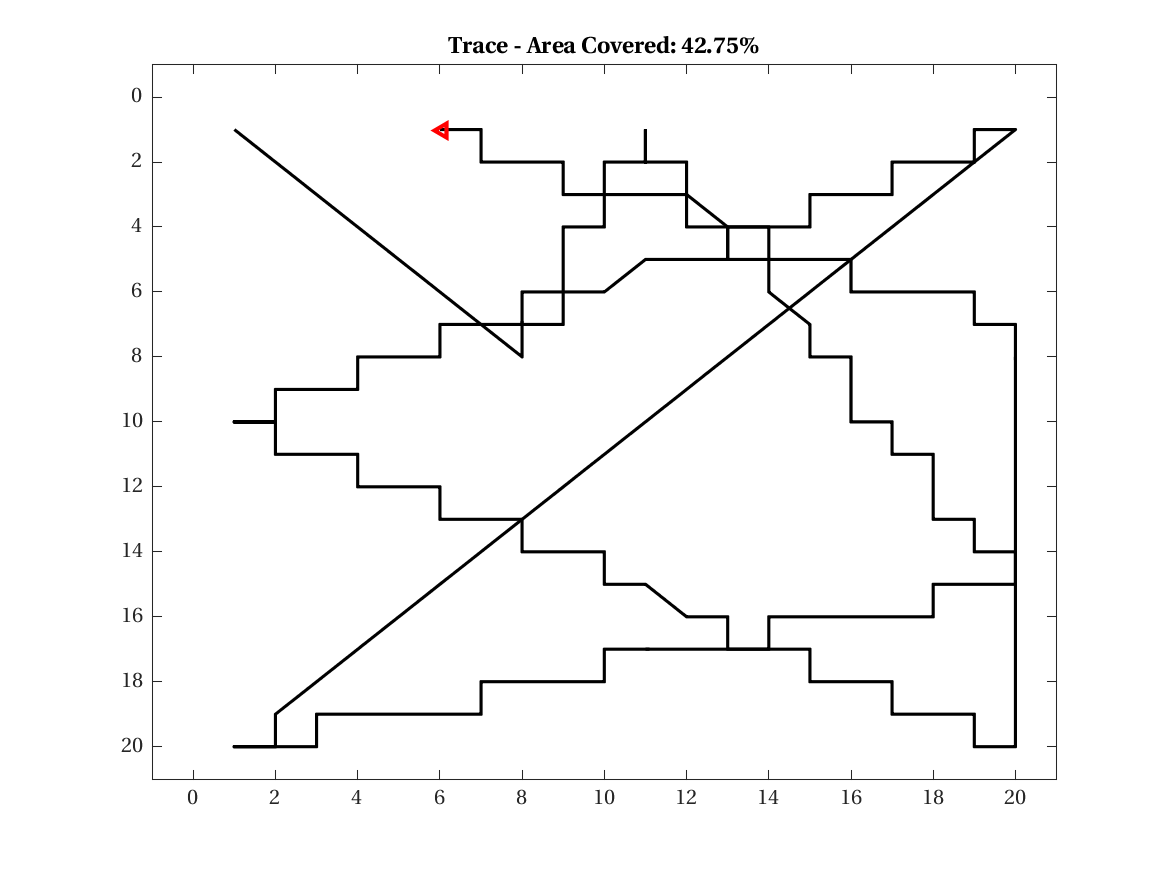
\includegraphics[width=\linewidth]{figures/hbresults/path_nhv_40p_20x20_sf_4_seed_2.png}
        \captionsetup{skip=0.20\baselineskip,size=footnotesize}
        \caption{Highest Variance}
    \end{subfigure}%
    \begin{subfigure}[t]{0.3333\textwidth}
        \centering
        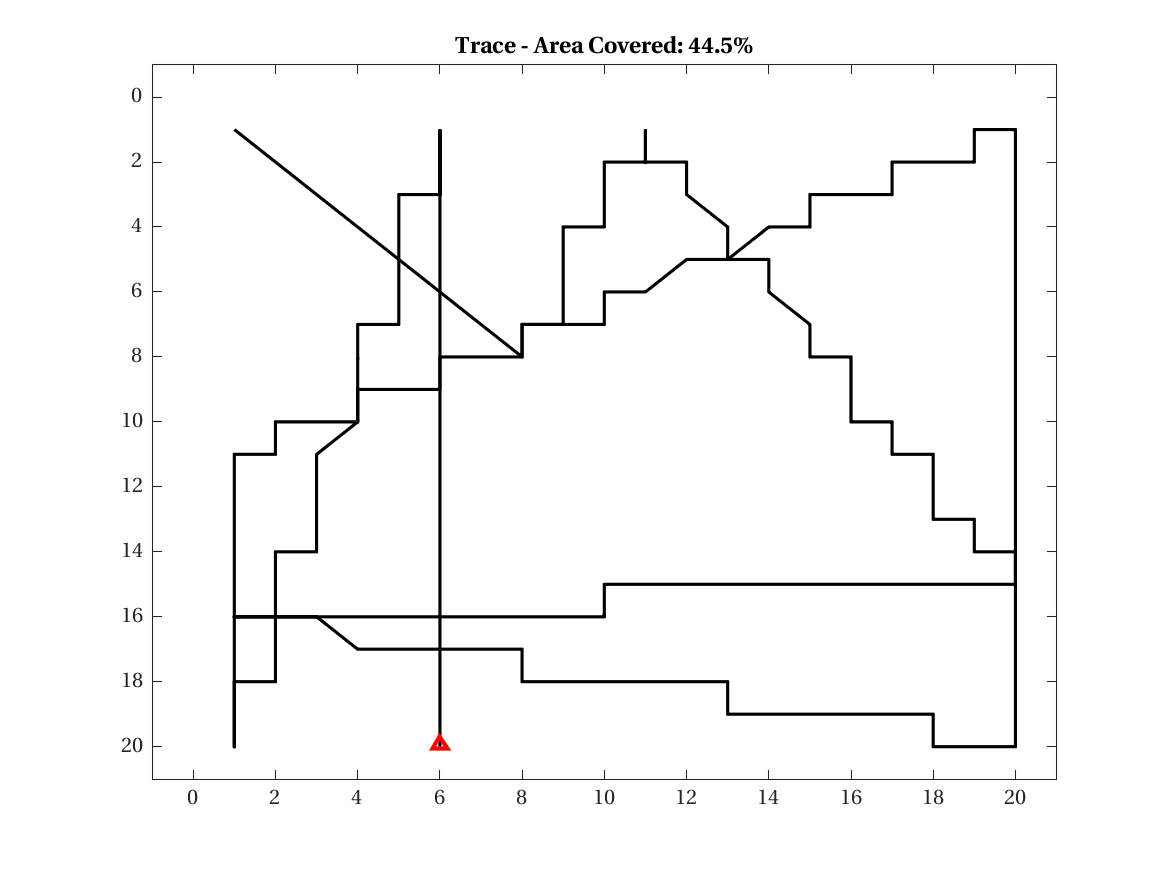
\includegraphics[width=\linewidth]{figures/hbresults/path_nnhv_40p_20x20_sf_4_seed_2.png}
        \captionsetup{skip=0.20\baselineskip,size=footnotesize}
        \caption{$N$ Highest Variance}
    \end{subfigure}%
    \begin{subfigure}[t]{0.3333\textwidth}
        \centering
        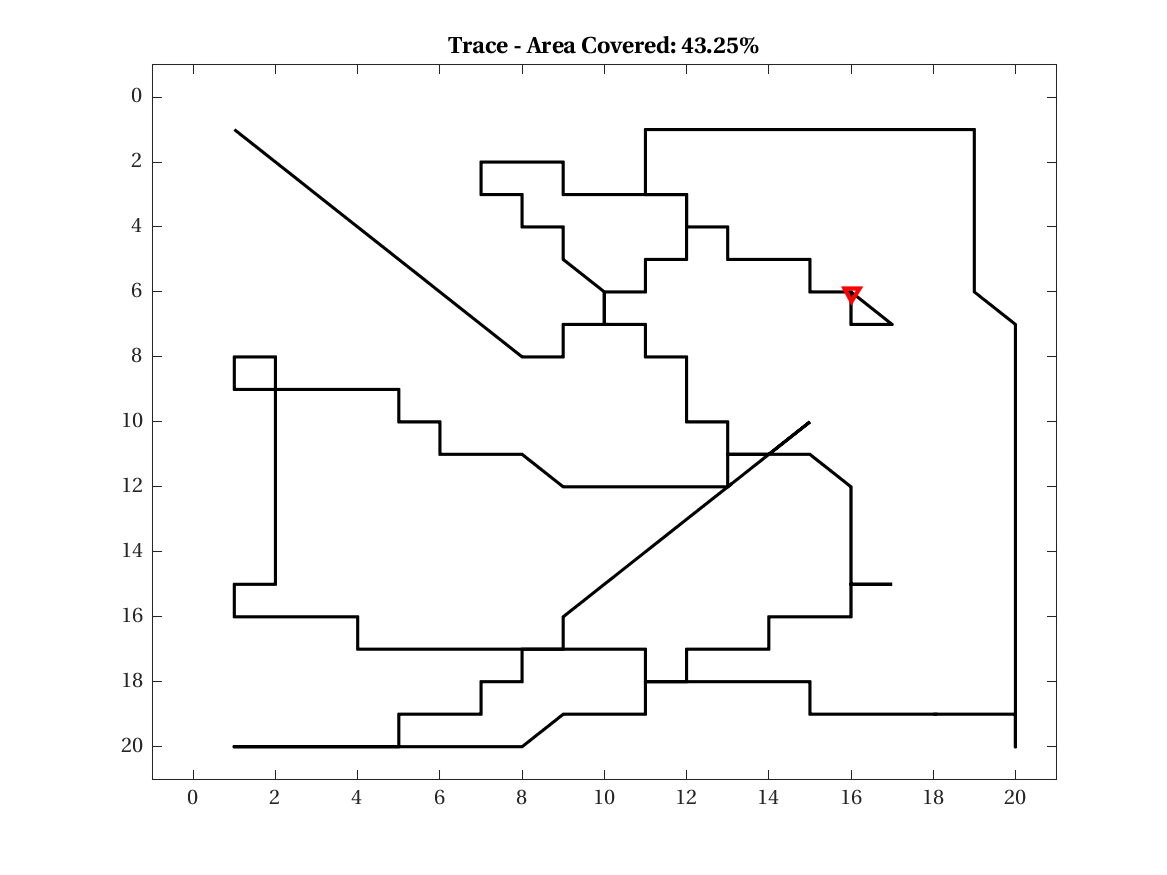
\includegraphics[width=\linewidth]{figures/hbresults/path_mc_40p_20x20_sf_4_seed_2.png}
        \captionsetup{skip=0.20\baselineskip,size=footnotesize}
        \caption{Monte Carlo}
    \end{subfigure}%
    \\
    \begin{subfigure}[t]{0.3333\textwidth}
        \centering
        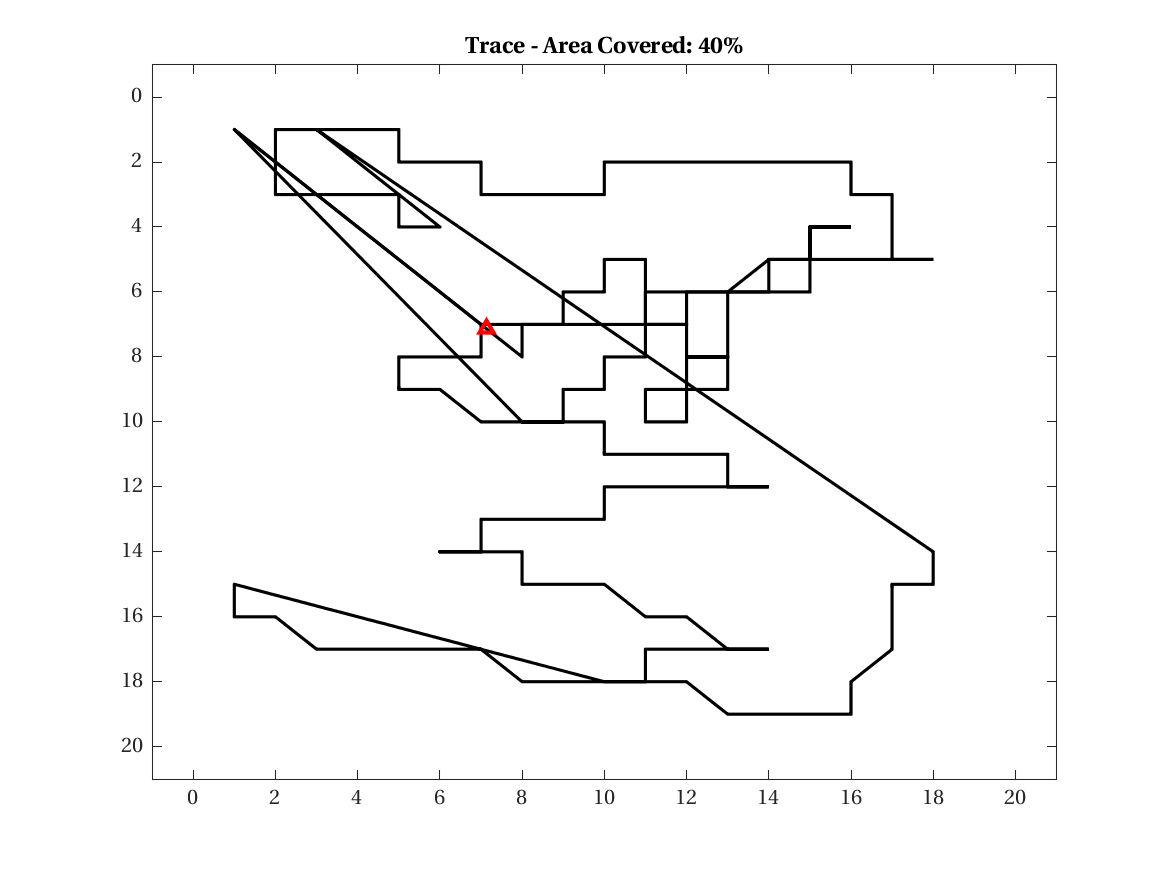
\includegraphics[width=\linewidth]{figures/hbresults/path_nbv_40p_20x20_sf_4_seed_2.png}
        \captionsetup{skip=0.20\baselineskip,size=footnotesize}
        \caption{Greedy NBV}
    \end{subfigure}%
    \begin{subfigure}[t]{0.3333\textwidth}
        \centering
        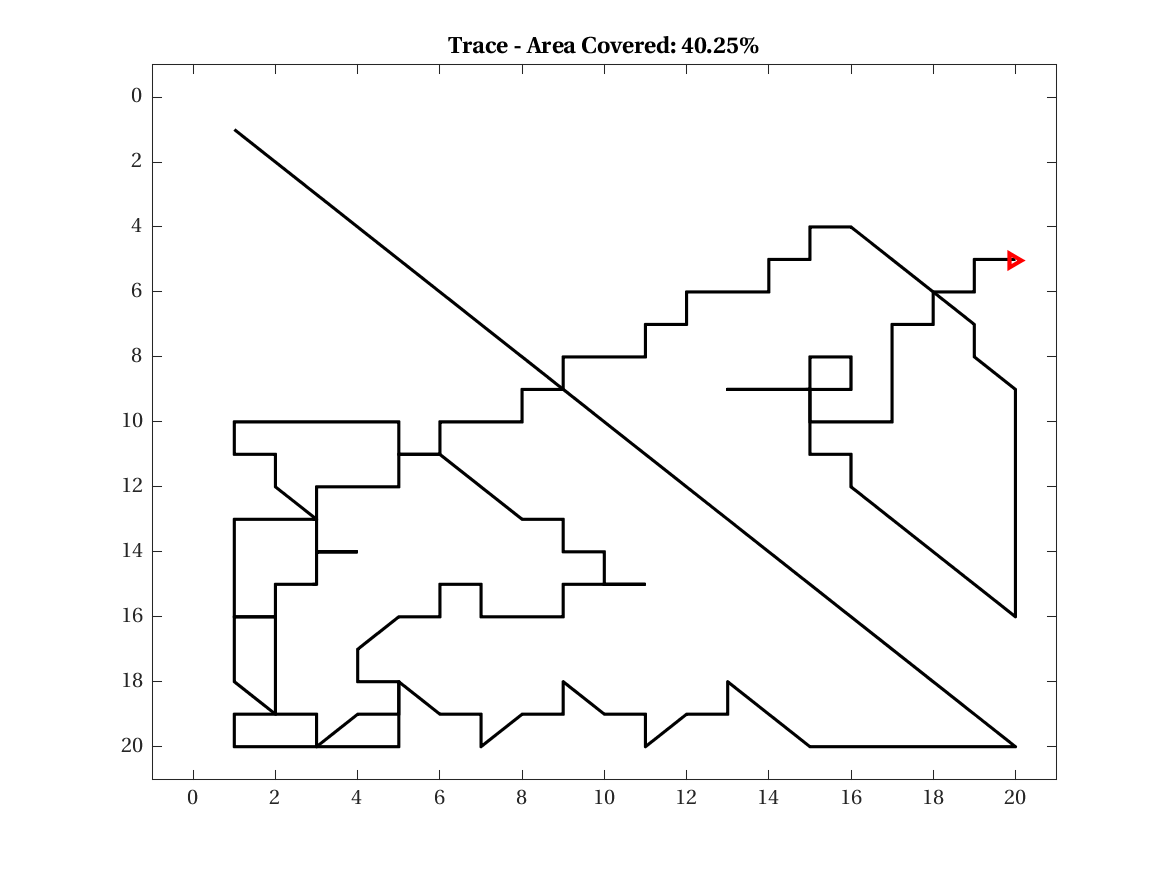
\includegraphics[width=\linewidth]{figures/hbresults/path_gradient_40p_20x20_sf_4_seed_2.png}
        \captionsetup{skip=0.20\baselineskip,size=footnotesize}
        \caption{Gradient Ascent}
    \end{subfigure}%
    \begin{subfigure}[t]{0.3333\textwidth}
        \centering
        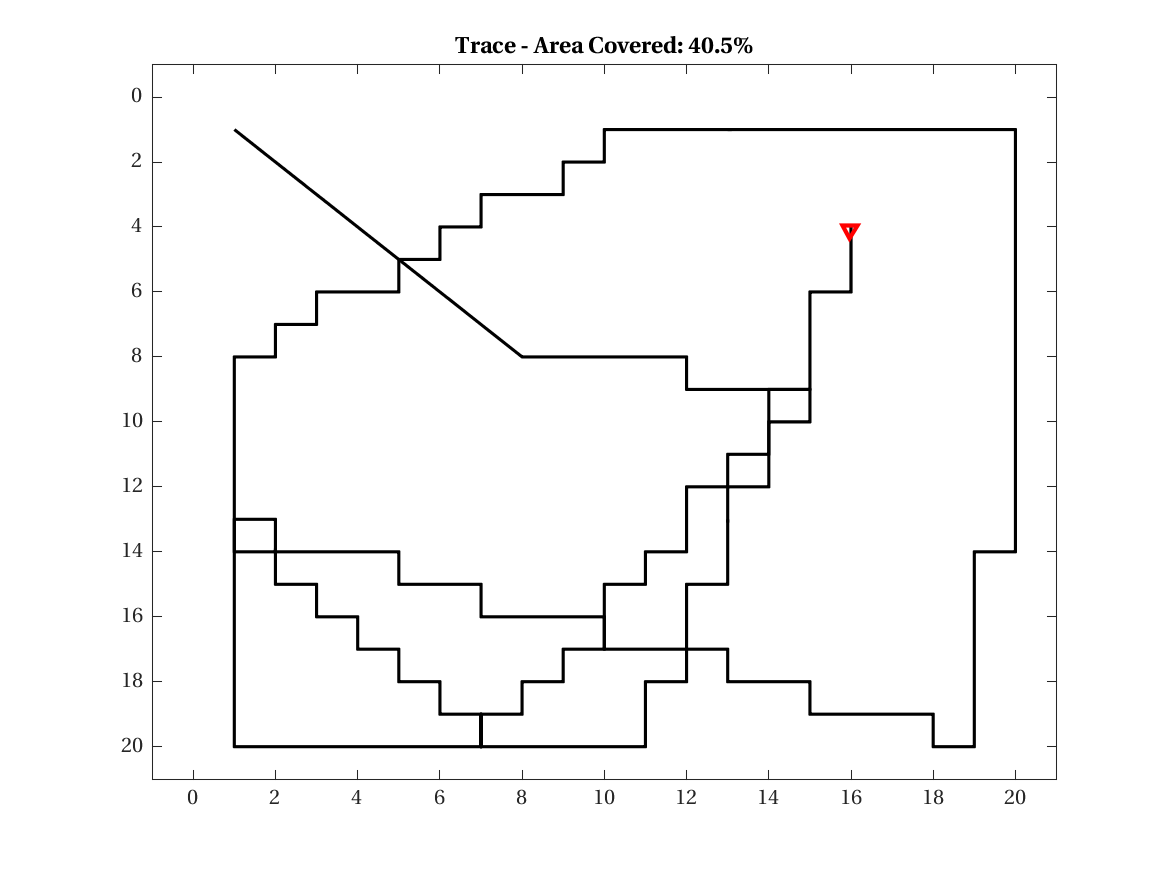
\includegraphics[width=\linewidth]{figures/hbresults/path_gr_40p_20x20_sf_4_seed_2.png}
        \captionsetup{skip=0.20\baselineskip,size=footnotesize}
        \caption{Gradient Range Ascent}
    \end{subfigure}%
    \\
    \begin{subfigure}[t]{0.3333\textwidth}
        \centering
        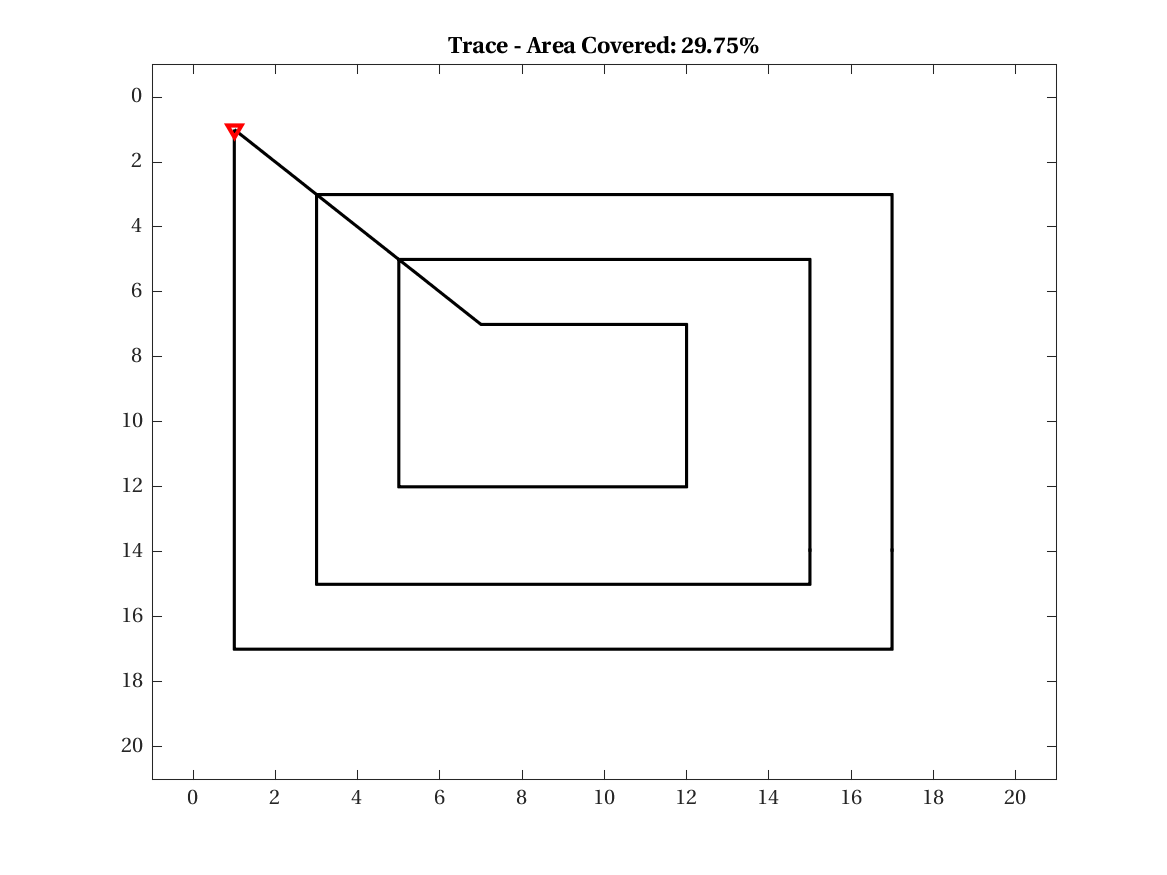
\includegraphics[width=\linewidth]{figures/hbresults/path_zz_40p_20x20_sf_4_seed_2.png}
        \captionsetup{skip=0.20\baselineskip,size=footnotesize}
        \caption{$ZZ_{30}$}
    \end{subfigure}%
    \captionsetup{skip=0.20\baselineskip}
    \caption{Exploration of a field of size $20 \times 20$, $\sigma_{field} = 4$, random seed 2.}
    \label{fig:nbvpathcomp}
\end{figure}

\begin{figure}[htb!]
    \centering
    \begin{subfigure}[t]{0.75\textwidth}
        \centering
        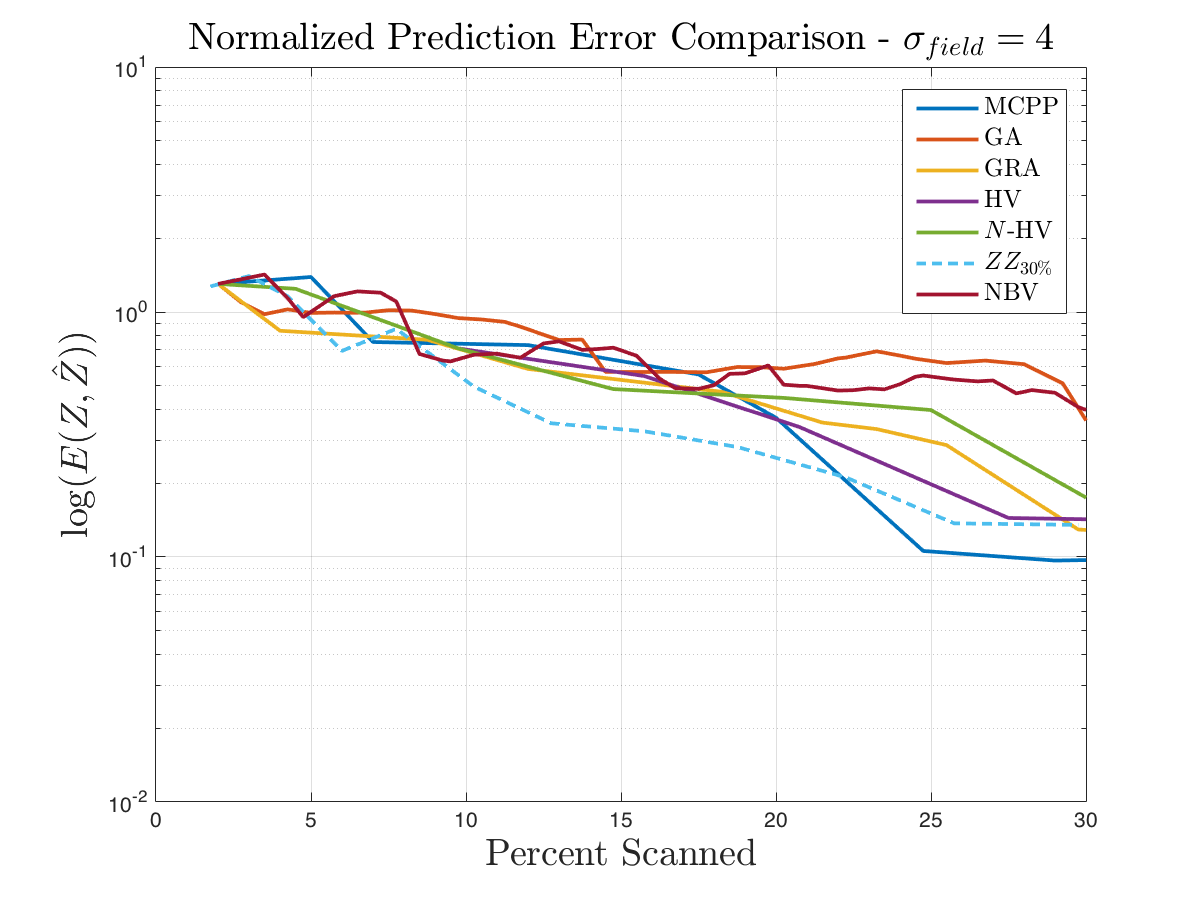
\includegraphics[width=\linewidth]{figures/results/normalized_errors_40p_20x20_sf_4_seed_2_app_10.png}
        \captionsetup{skip=0.20\baselineskip,size=footnotesize}
        \caption{Normalized prediction errors for each method.}
    \end{subfigure}%
    \\
    \begin{subfigure}[t]{0.75\textwidth}
        \centering
        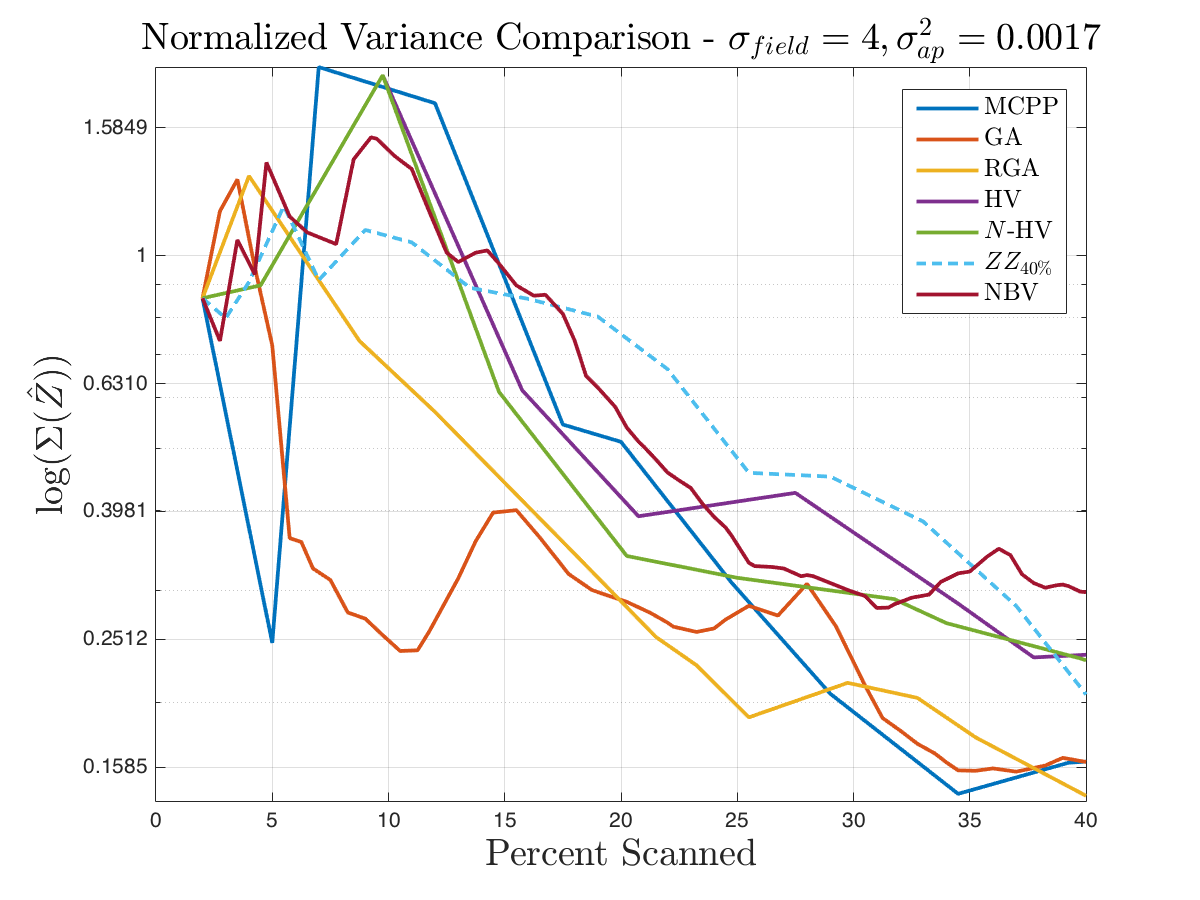
\includegraphics[width=\linewidth]{figures/results/normalized_variances_40p_20x20_sf_4_seed_2_app_10.png}
        \captionsetup{skip=0.20\baselineskip,size=footnotesize}
        \caption{Normalized prediction variances for each method.}
    \end{subfigure}%
    \captionsetup{skip=0.20\baselineskip}
    \caption{Prediction error and variances for an exploration of a field of size $20 \times 20$, $\sigma_{field} = 4$, random seed 2.}
    \label{fig:nbvcomp}
\end{figure}

\FloatBarrier
\clearpage

\section{High Spatial Autocorrelation Results}
The methods will be compared on target fields generated with an autocorrelation factor, $\sigma_{field}$, equal to the field width. A Gaussian filter $G(x,y,100)$ (Equation \ref{eq:gauss_filt}), is convolved with all points on the field.

\begin{figure}[htb!]
    \centering
    \begin{subfigure}[t]{0.3333\textwidth}
        \centering
        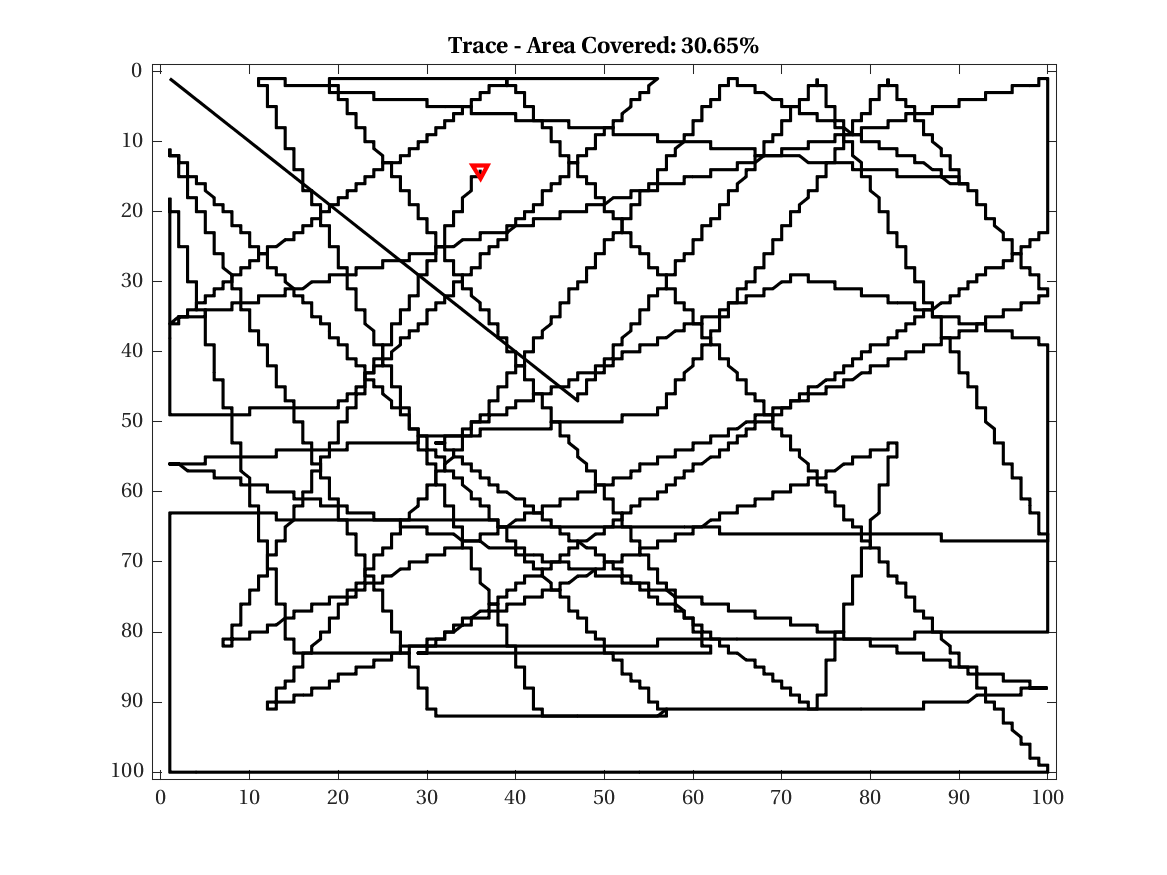
\includegraphics[width=\linewidth]{figures/hbresults/path_nhv_30p_100x100_sf_100_seed_2.png}
        \captionsetup{skip=0.20\baselineskip,size=footnotesize}
        \caption{Highest Variance}
    \end{subfigure}%
    \begin{subfigure}[t]{0.3333\textwidth}
        \centering
        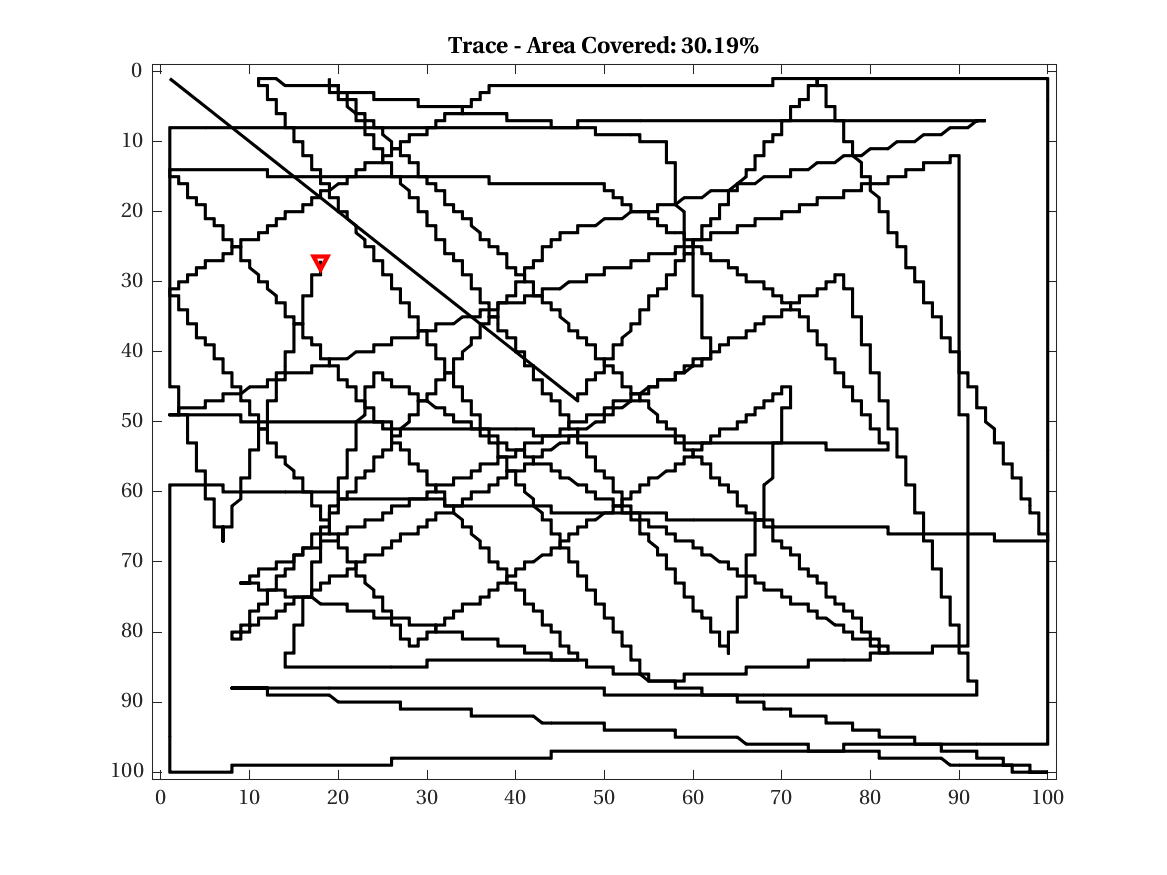
\includegraphics[width=\linewidth]{figures/hbresults/path_nnhv_30p_100x100_sf_100_seed_2.png}
        \captionsetup{skip=0.20\baselineskip,size=footnotesize}
        \caption{$N$ Highest Variance}
    \end{subfigure}%
    \begin{subfigure}[t]{0.3333\textwidth}
        \centering
        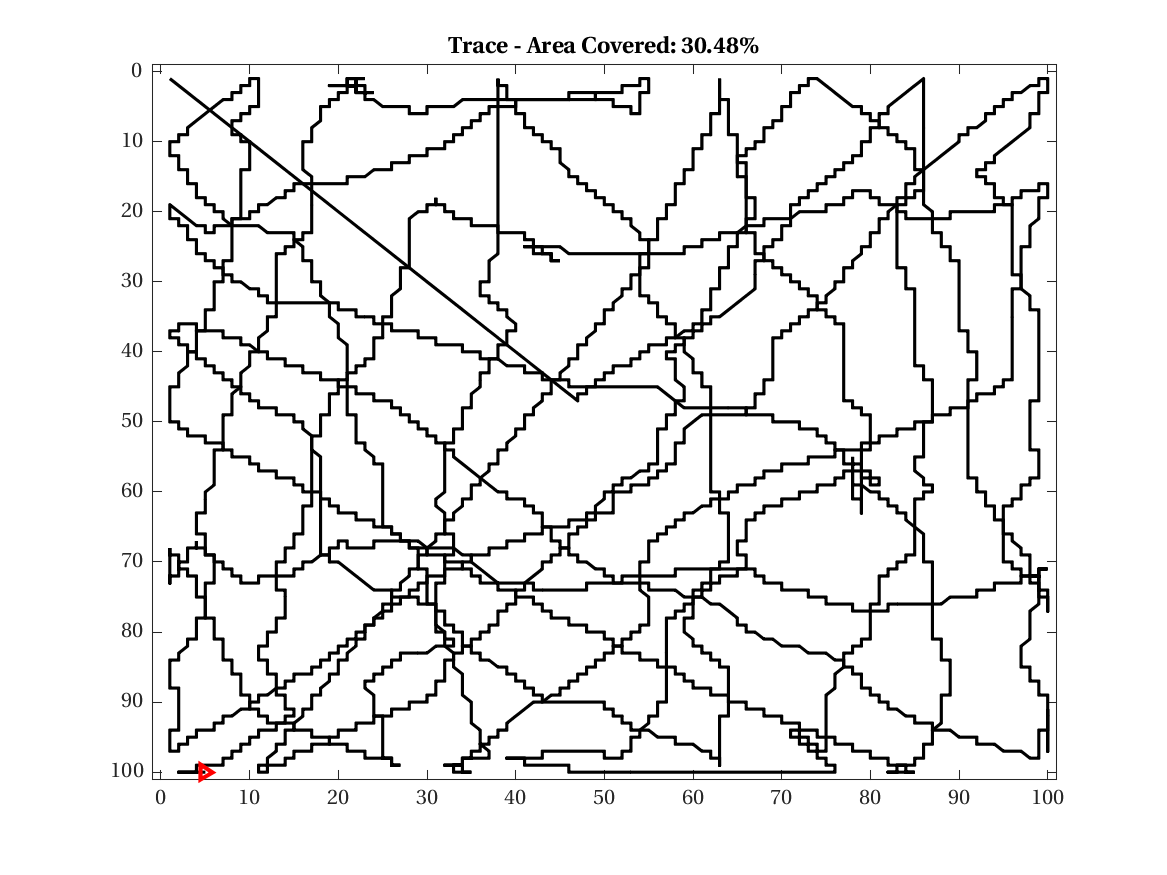
\includegraphics[width=\linewidth]{figures/hbresults/path_mc_30p_100x100_sf_100_seed_2.png}
        \captionsetup{skip=0.20\baselineskip,size=footnotesize}
        \caption{Monte Carlo}
    \end{subfigure}%
    \\
    \begin{subfigure}[t]{0.3333\textwidth}
        \centering
        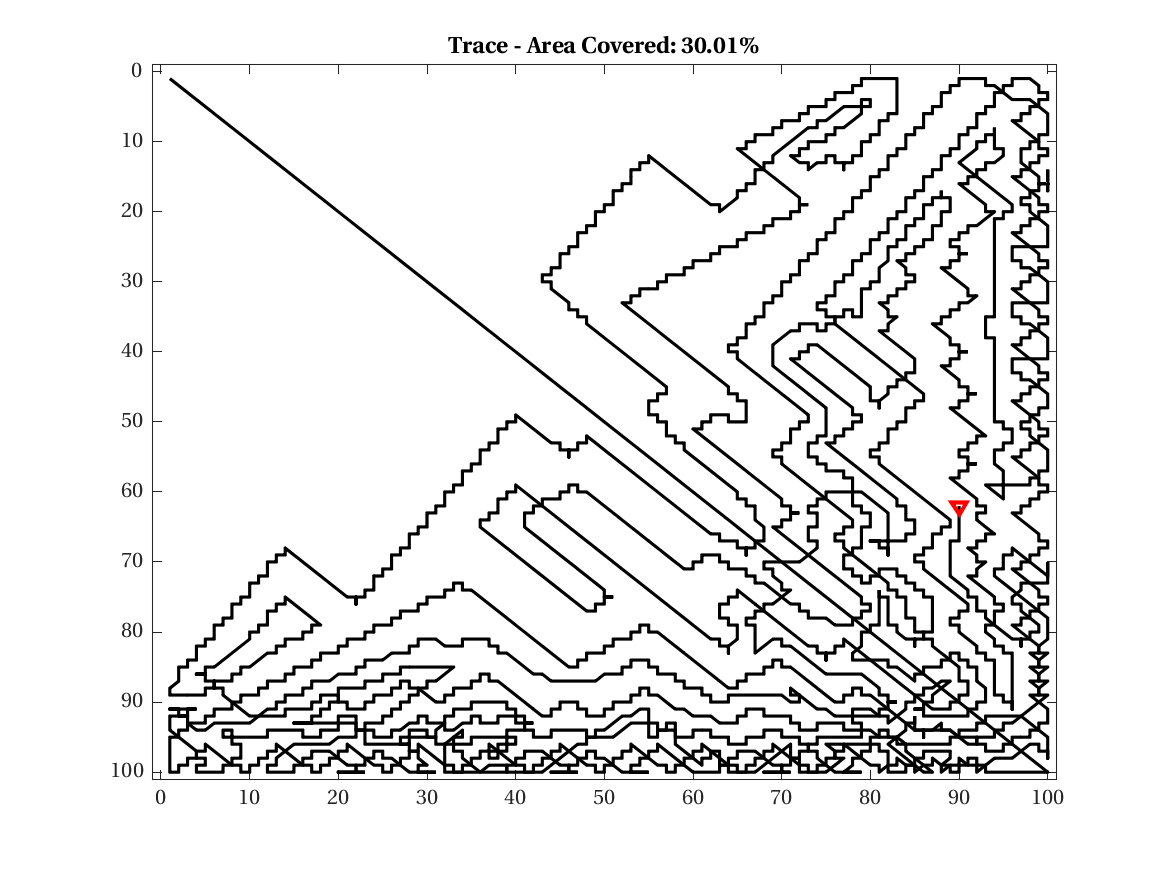
\includegraphics[width=\linewidth]{figures/hbresults/path_gradient_30p_100x100_sf_100_seed_2.png}
        \captionsetup{skip=0.20\baselineskip,size=footnotesize}
        \caption{Gradient Ascent}
    \end{subfigure}%
    \begin{subfigure}[t]{0.3333\textwidth}
        \centering
        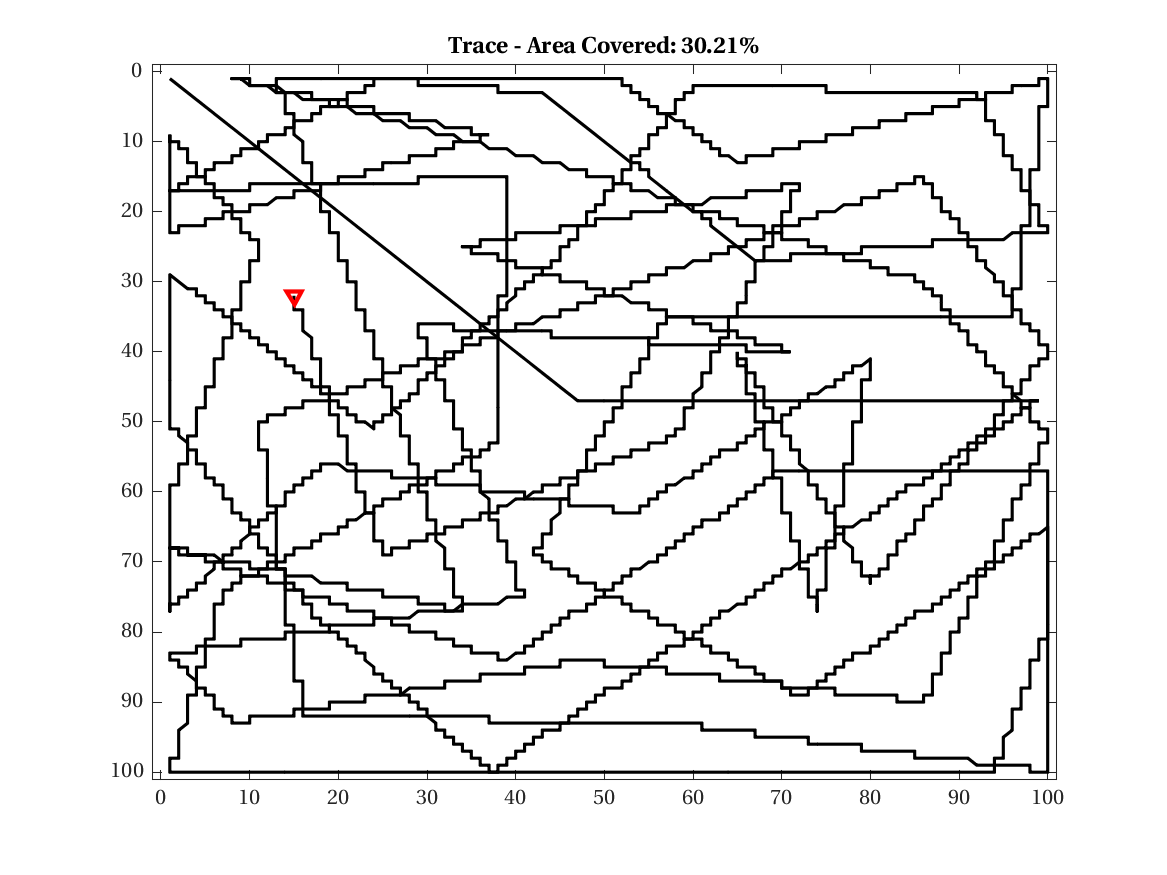
\includegraphics[width=\linewidth]{figures/hbresults/path_gr_30p_100x100_sf_100_seed_2.png}
        \captionsetup{skip=0.20\baselineskip,size=footnotesize}
        \caption{Gradient Range Ascent}
    \end{subfigure}%
    \\
    \begin{subfigure}[t]{0.3333\textwidth}
        \centering
        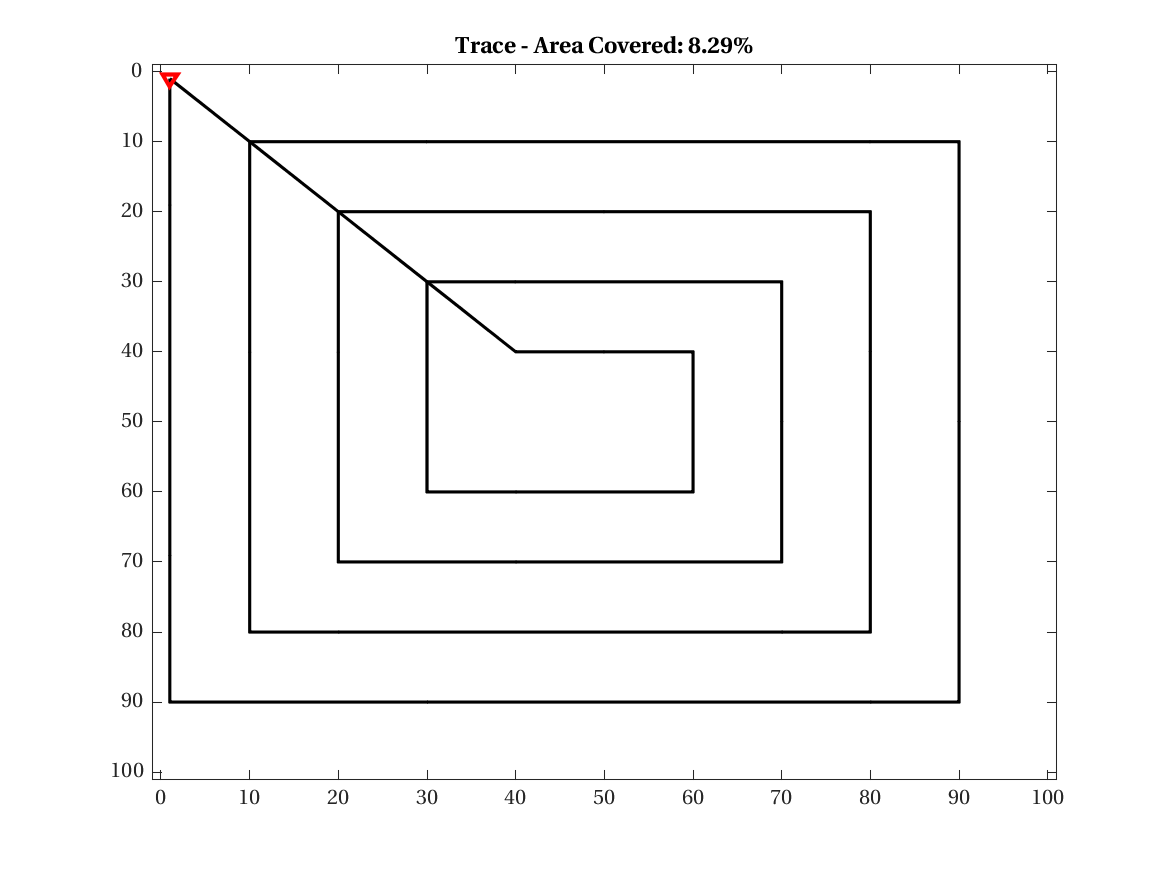
\includegraphics[width=\linewidth]{figures/hbresults/path_zz_10p_100x100_sf_100_seed_2.png}
        \captionsetup{skip=0.20\baselineskip,size=footnotesize}
        \caption{$ZZ_{10}$}
    \end{subfigure}%
    \begin{subfigure}[t]{0.3333\textwidth}
        \centering
        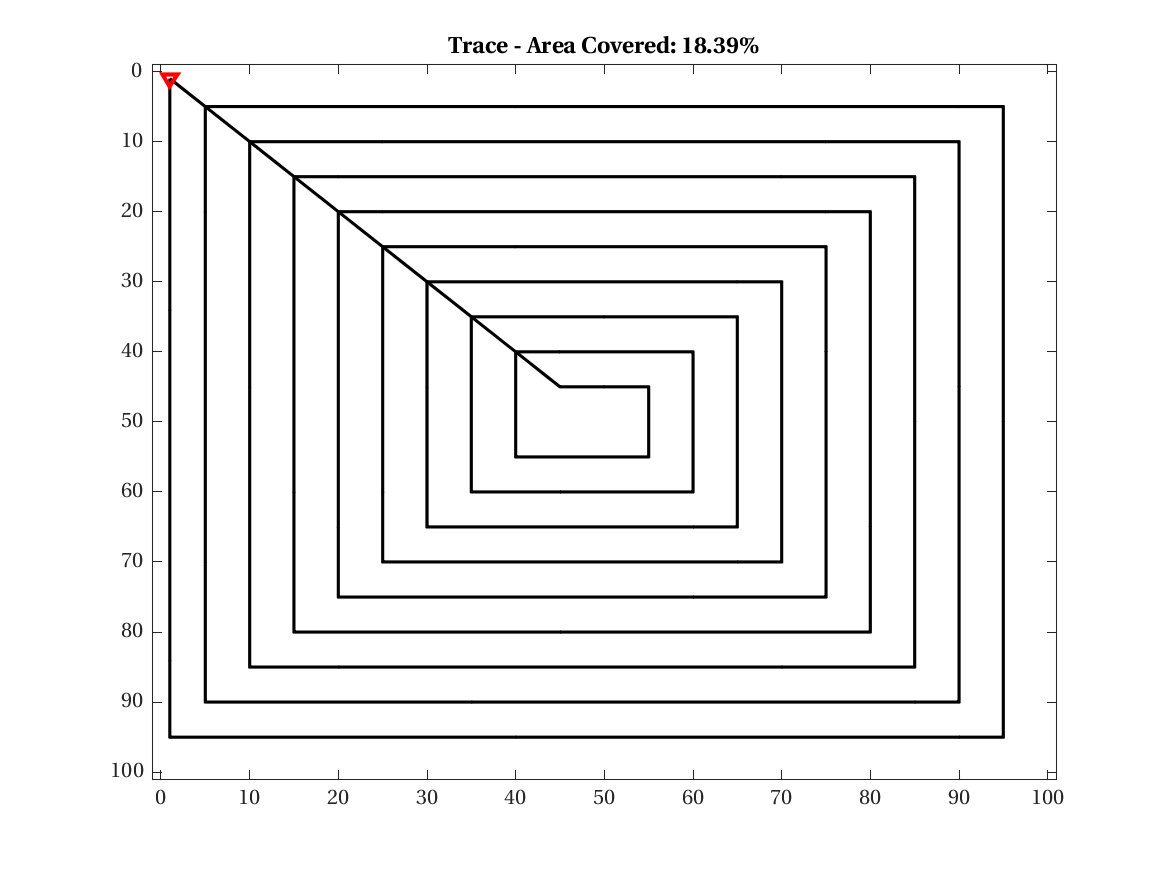
\includegraphics[width=\linewidth]{figures/hbresults/path_zz_20p_100x100_sf_100_seed_2.png}
        \captionsetup{skip=0.20\baselineskip,size=footnotesize}
        \caption{$ZZ_{20}$}
    \end{subfigure}%
    \begin{subfigure}[t]{0.3333\textwidth}
        \centering
        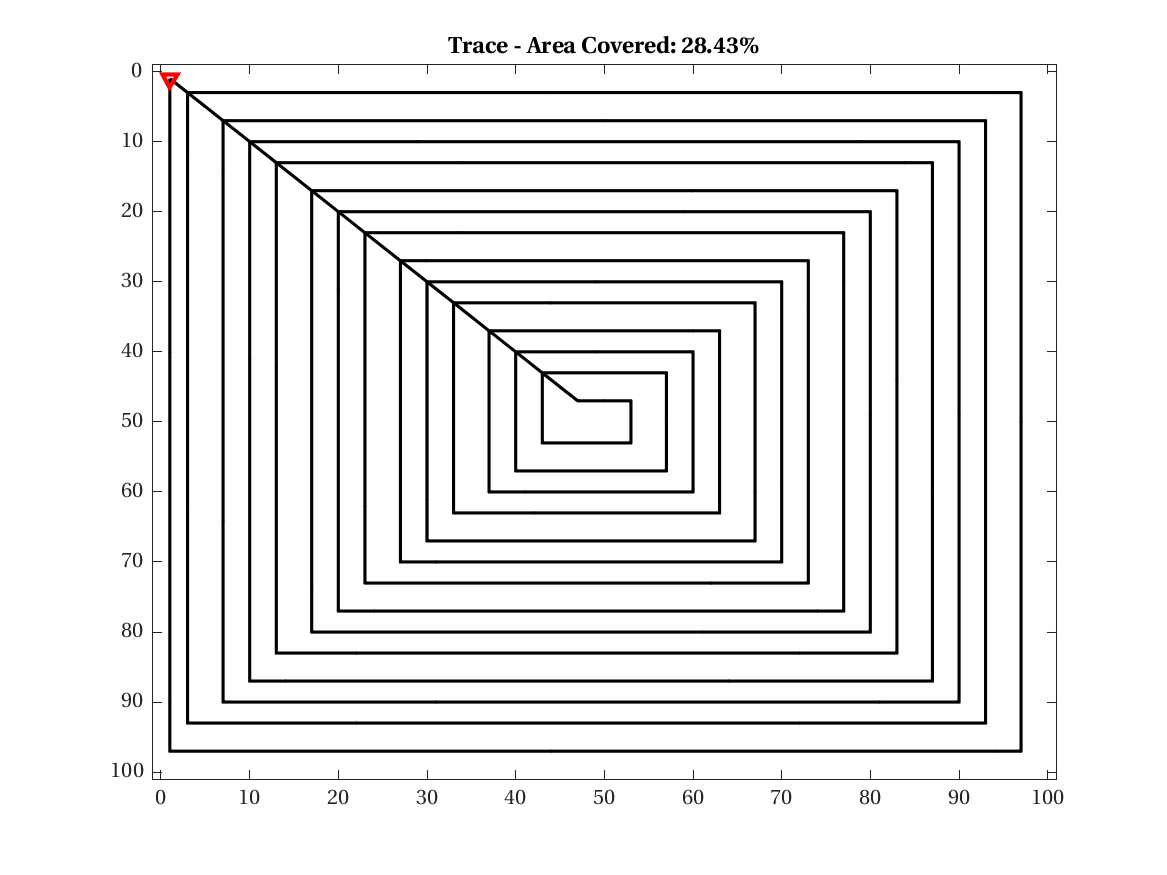
\includegraphics[width=\linewidth]{figures/hbresults/path_zz_30p_100x100_sf_100_seed_2.png}
        \captionsetup{skip=0.20\baselineskip,size=footnotesize}
        \caption{$ZZ_{30}$}
    \end{subfigure}%
    \captionsetup{skip=0.20\baselineskip}
    \caption{Exploration of a field of size $100 \times 100$, $\sigma_{field} = 100$, random seed 2.}
    \label{fig:sf100}
\end{figure}

\begin{figure}[htb!]
    \centering
    \begin{subfigure}[t]{0.75\textwidth}
        \centering
        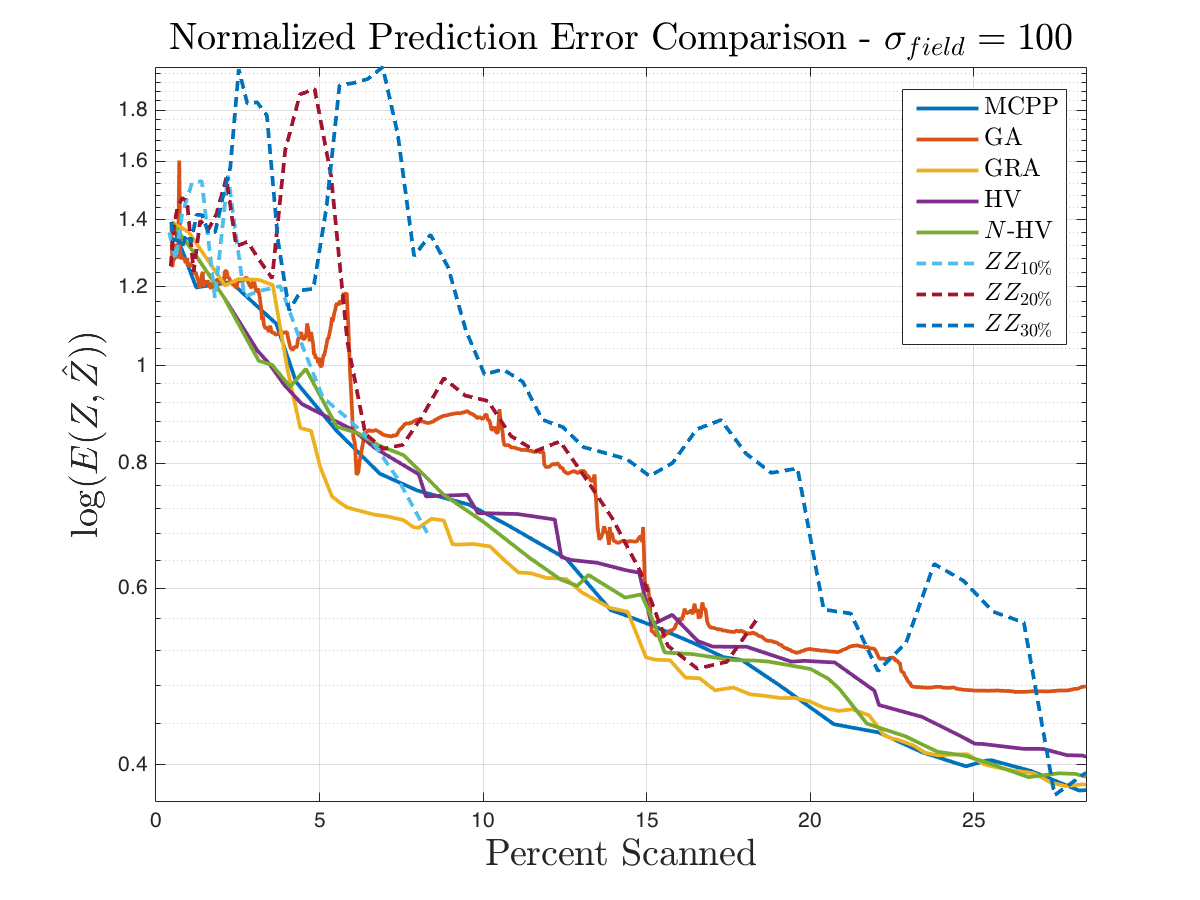
\includegraphics[width=\linewidth]{figures/results/normalized_errors_30p_100x100_sf_100_seed_2_app_50.png}
        \captionsetup{skip=0.20\baselineskip,size=footnotesize}
        \caption{Normalized prediction errors for each method.}
    \end{subfigure}%
    \\
    \begin{subfigure}[t]{0.75\textwidth}
        \centering
        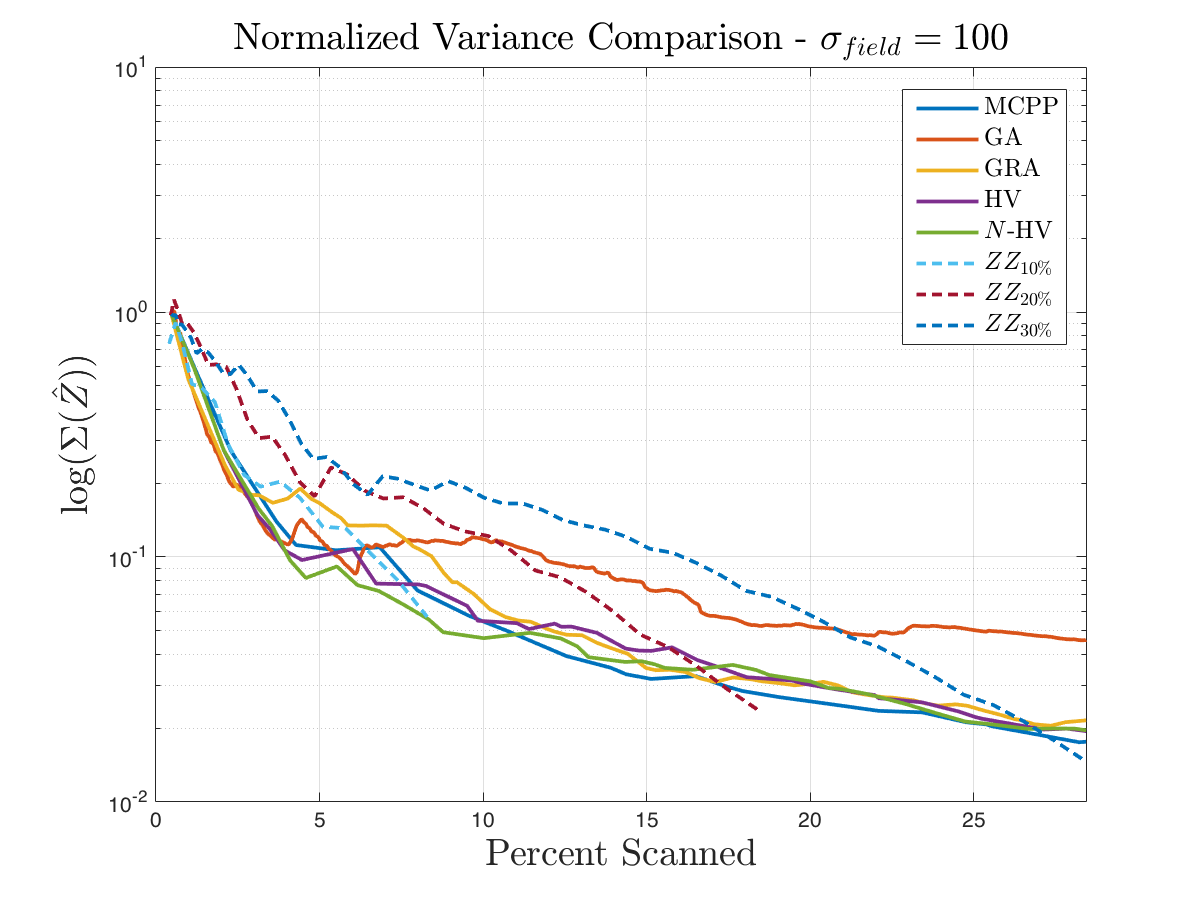
\includegraphics[width=\linewidth]{figures/results/normalized_variances_30p_100x100_sf_100_seed_2_app_50.png}
        \captionsetup{skip=0.20\baselineskip,size=footnotesize}
        \caption{Normalized prediction variances for each method.}
    \end{subfigure}%
    \captionsetup{skip=0.20\baselineskip}
    \caption{Prediction error and variances for an exploration of a field of size $100 \times 100$, $\sigma_{field} = 100$, random seed 2.}
    \label{fig:errvar100}
\end{figure}

\FloatBarrier
\clearpage

\section{Half Width Spatial Autocorrelation Results}
The methods will be compared on target fields generated with an autocorrelation factor, $\sigma_{field}$, equal to the half of the target field's width. A Gaussian filter $G(x,y,50)$ (Equation \ref{eq:gauss_filt}), is convolved with all points on the field.

\begin{figure}[htb!]
    \centering
    \begin{subfigure}[t]{0.3333\textwidth}
        \centering
        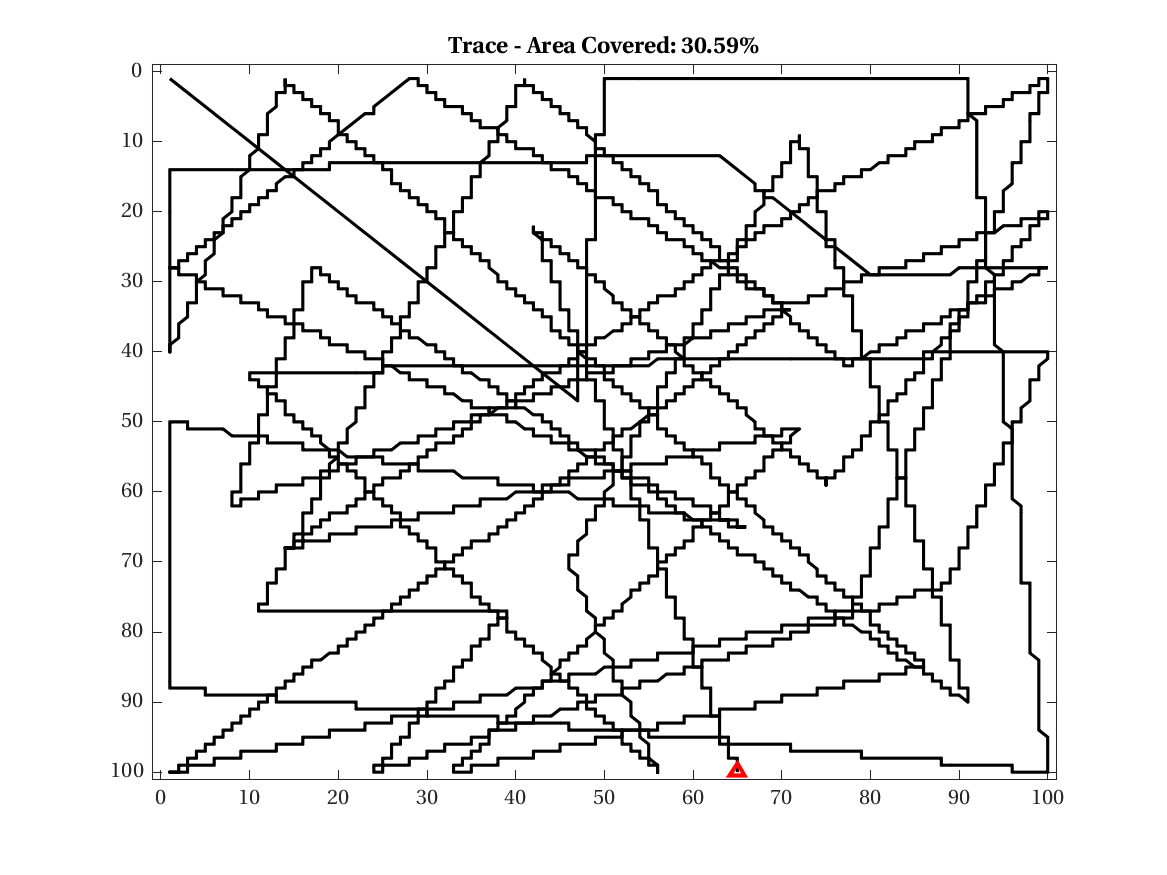
\includegraphics[width=\linewidth]{figures/hbresults/path_nhv_30p_100x100_sf_50_seed_2.png}
        \captionsetup{skip=0.20\baselineskip,size=footnotesize}
        \caption{Highest Variance}
    \end{subfigure}%
    \begin{subfigure}[t]{0.3333\textwidth}
        \centering
        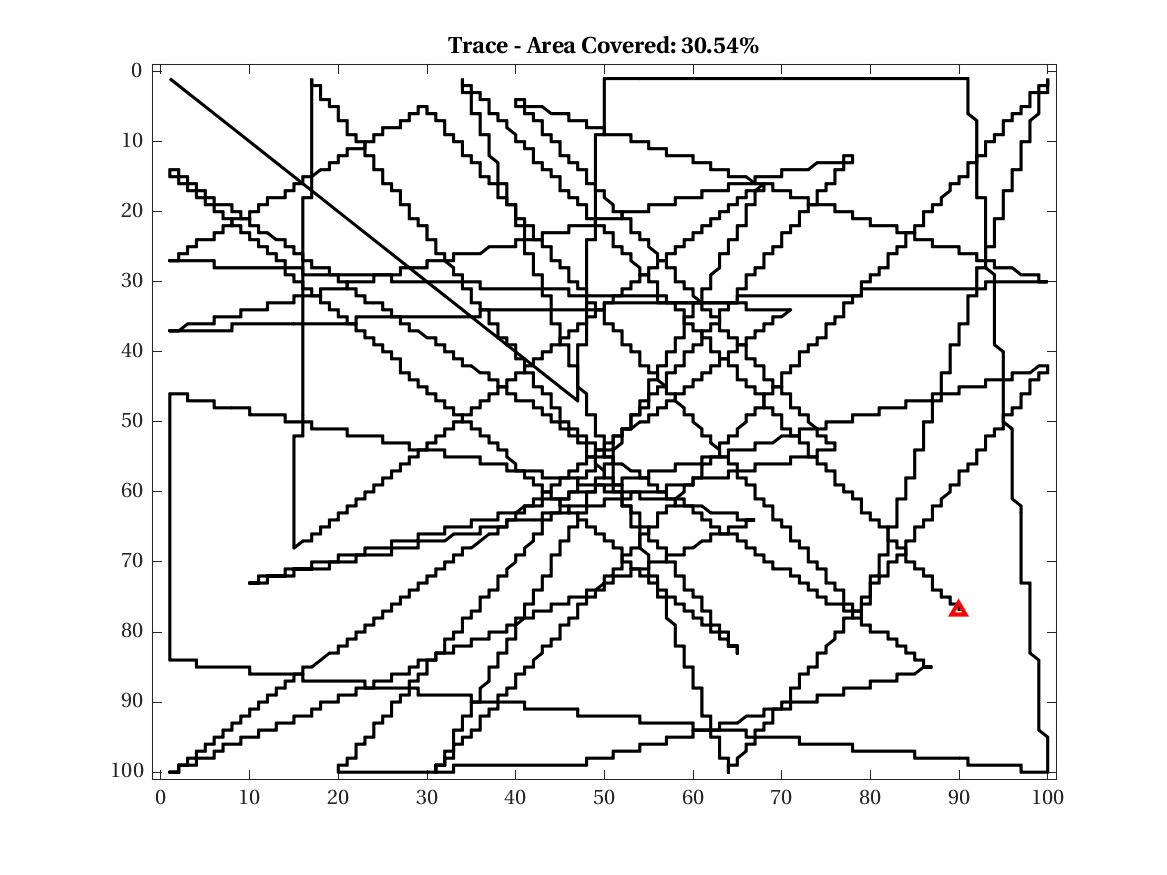
\includegraphics[width=\linewidth]{figures/hbresults/path_nnhv_30p_100x100_sf_50_seed_2.png}
        \captionsetup{skip=0.20\baselineskip,size=footnotesize}
        \caption{$N$ Highest Variance}
    \end{subfigure}%
    \begin{subfigure}[t]{0.3333\textwidth}
        \centering
        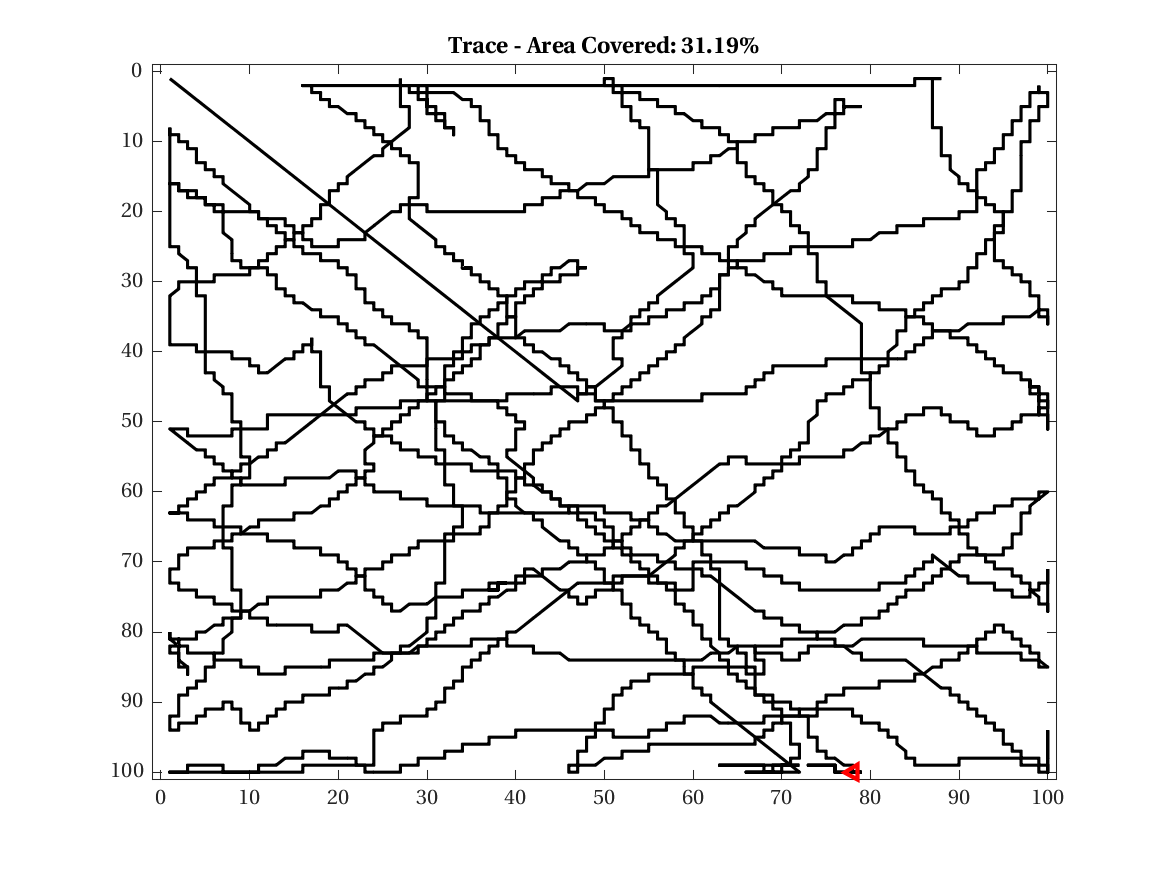
\includegraphics[width=\linewidth]{figures/hbresults/path_mc_30p_100x100_sf_50_seed_2.png}
        \captionsetup{skip=0.20\baselineskip,size=footnotesize}
        \caption{Monte Carlo}
    \end{subfigure}%
    \\
    \begin{subfigure}[t]{0.3333\textwidth}
        \centering
        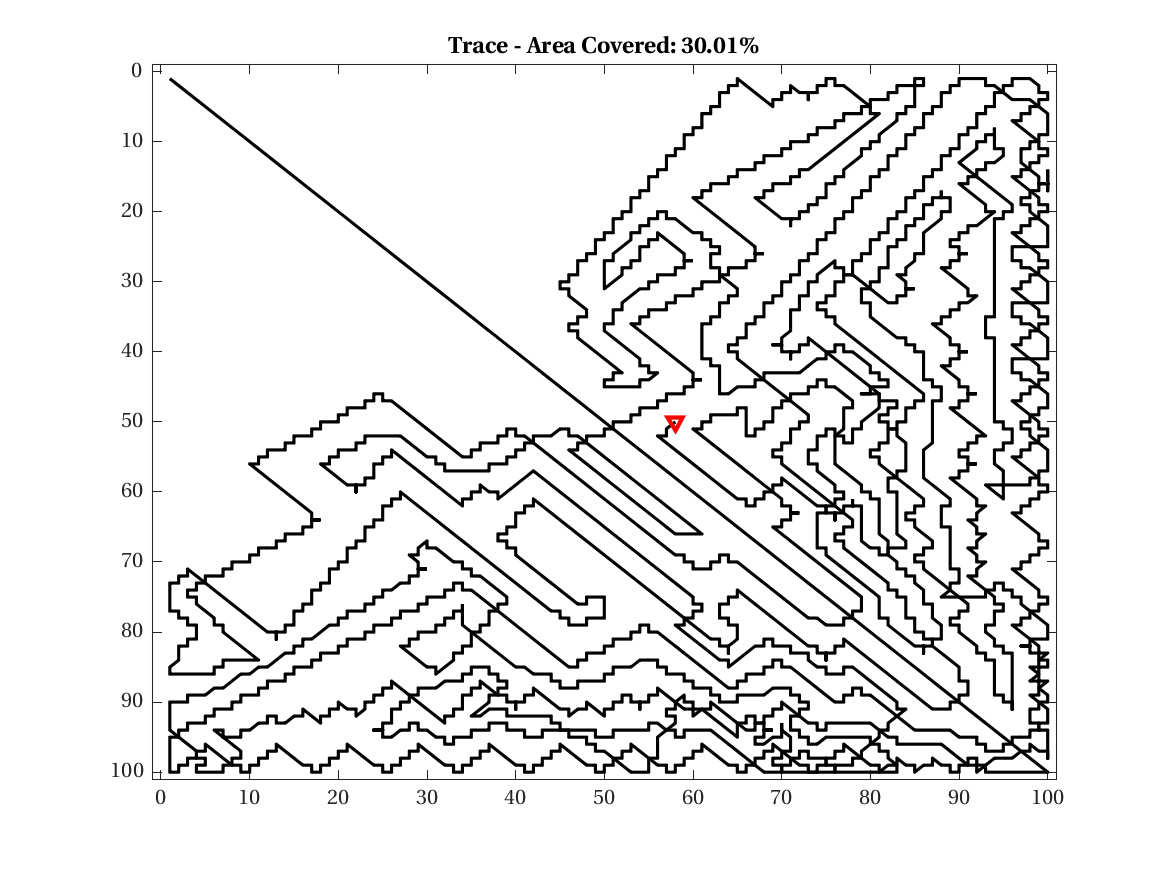
\includegraphics[width=\linewidth]{figures/hbresults/path_gradient_30p_100x100_sf_50_seed_2.png}
        \captionsetup{skip=0.20\baselineskip,size=footnotesize}
        \caption{Gradient Ascent}
    \end{subfigure}%
    \begin{subfigure}[t]{0.3333\textwidth}
        \centering
        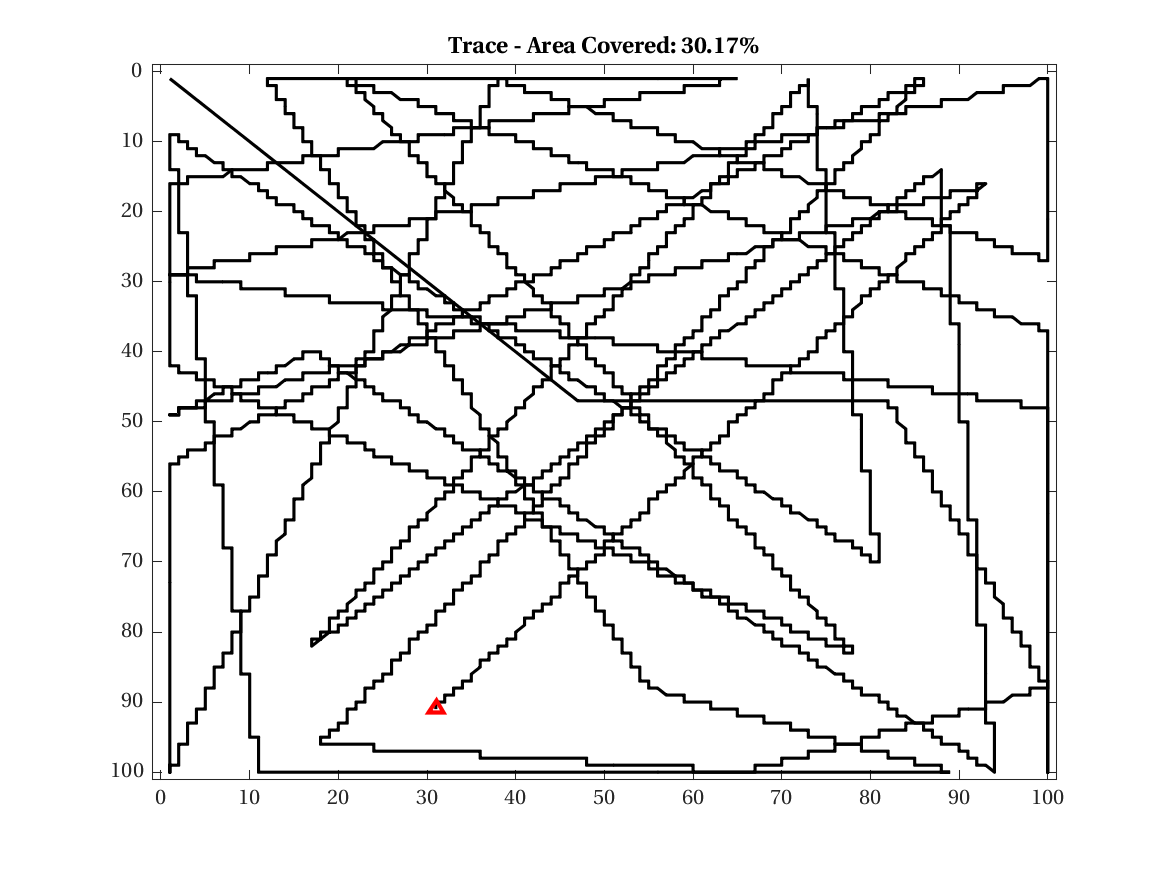
\includegraphics[width=\linewidth]{figures/hbresults/path_gr_30p_100x100_sf_50_seed_2.png}
        \captionsetup{skip=0.20\baselineskip,size=footnotesize}
        \caption{Gradient Range Ascent}
    \end{subfigure}%
    \\
    \begin{subfigure}[t]{0.3333\textwidth}
        \centering
        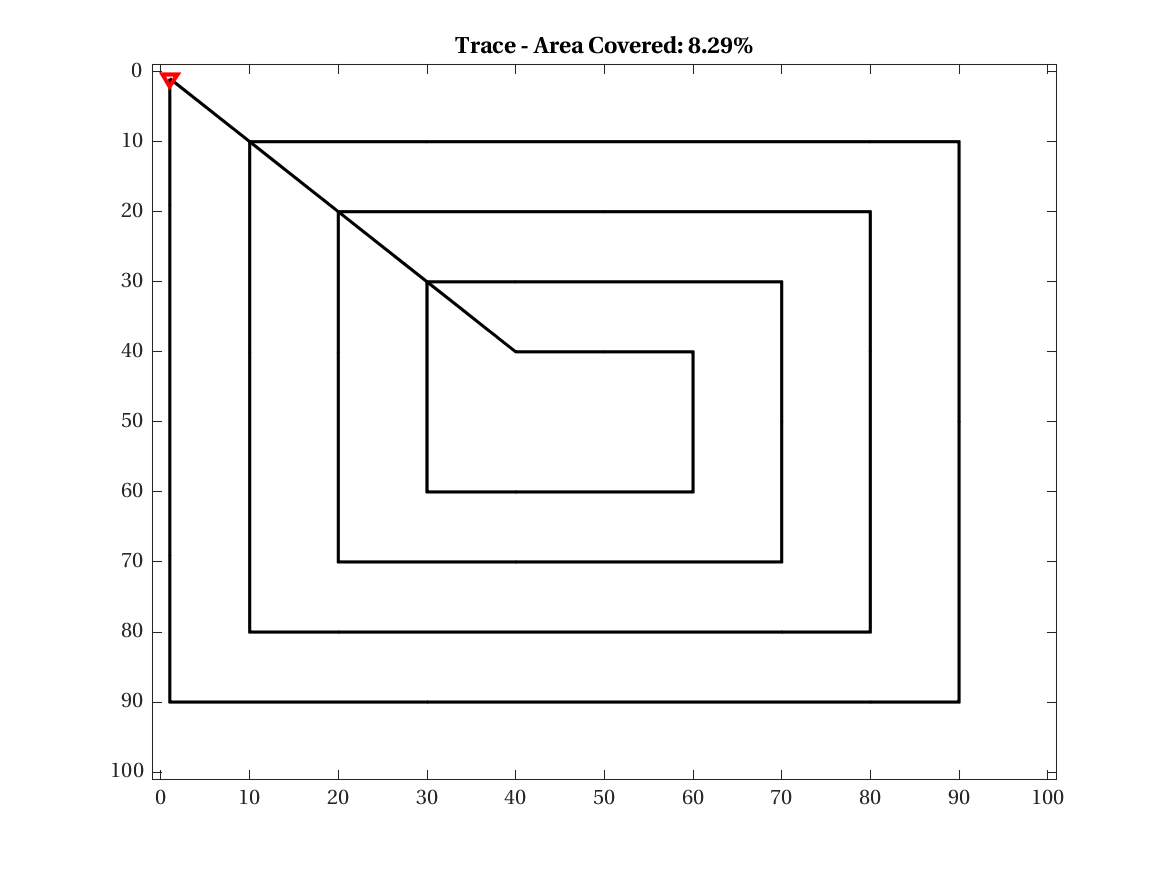
\includegraphics[width=\linewidth]{figures/hbresults/path_zz_10p_100x100_sf_50_seed_2.png}
        \captionsetup{skip=0.20\baselineskip,size=footnotesize}
        \caption{$ZZ_{10}$}
    \end{subfigure}%
    \begin{subfigure}[t]{0.3333\textwidth}
        \centering
        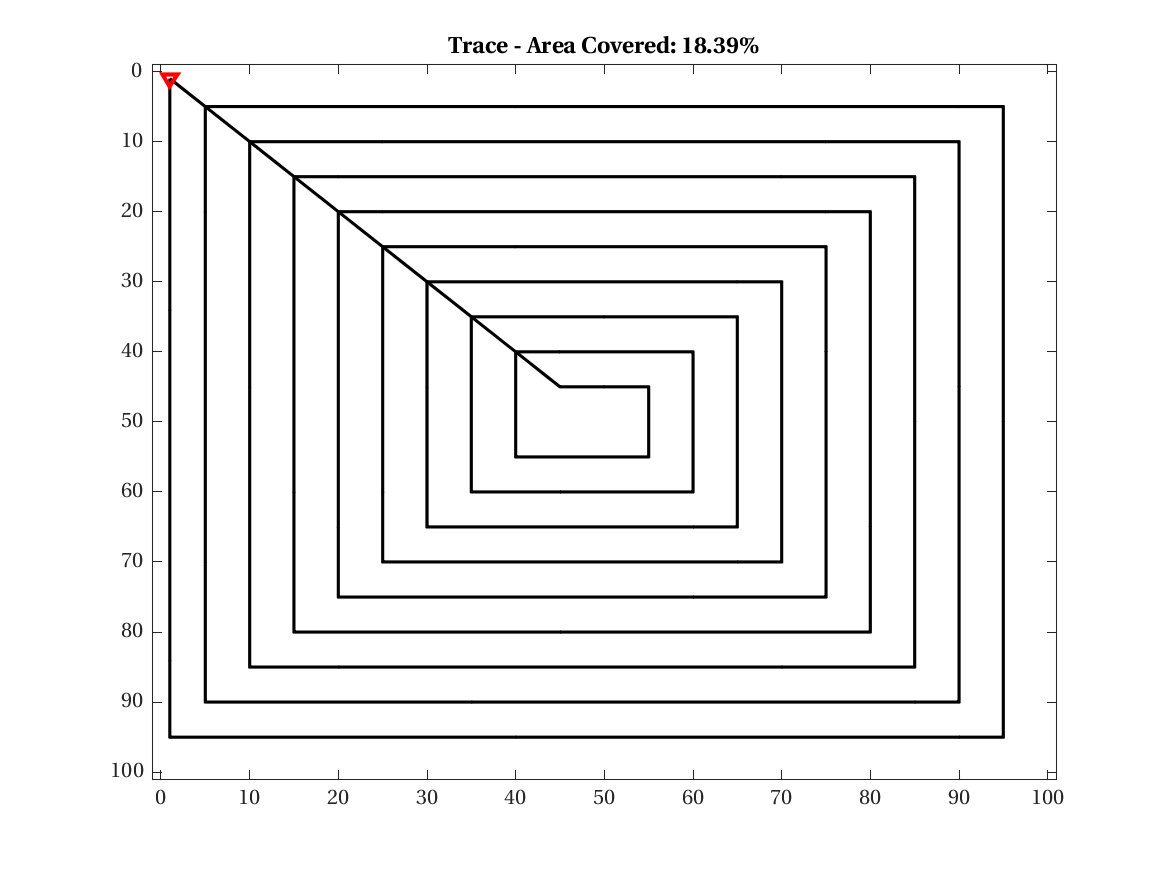
\includegraphics[width=\linewidth]{figures/hbresults/path_zz_20p_100x100_sf_50_seed_2.png}
        \captionsetup{skip=0.20\baselineskip,size=footnotesize}
        \caption{$ZZ_{20}$}
    \end{subfigure}%
    \begin{subfigure}[t]{0.3333\textwidth}
        \centering
        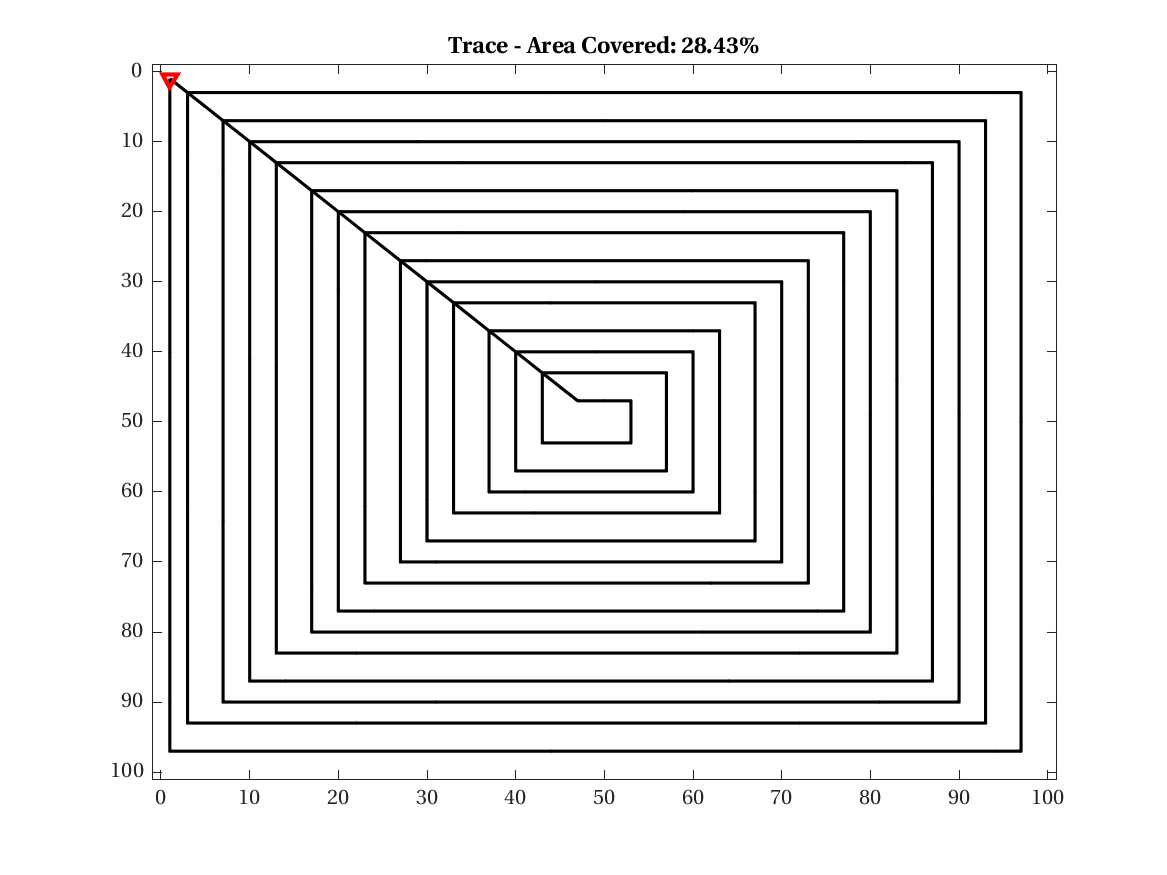
\includegraphics[width=\linewidth]{figures/hbresults/path_zz_30p_100x100_sf_50_seed_2.png}
        \captionsetup{skip=0.20\baselineskip,size=footnotesize}
        \caption{$ZZ_{30}$}
    \end{subfigure}%
    \captionsetup{skip=0.20\baselineskip}
    \caption{Exploration of a field of size $100 \times 100$, $\sigma_{field} = \frac{w}{2} = 50$, random seed 2.}
    \label{fig:sf50}
\end{figure}

\begin{figure}[htb!]
    \centering
    \begin{subfigure}[t]{0.75\textwidth}
        \centering
        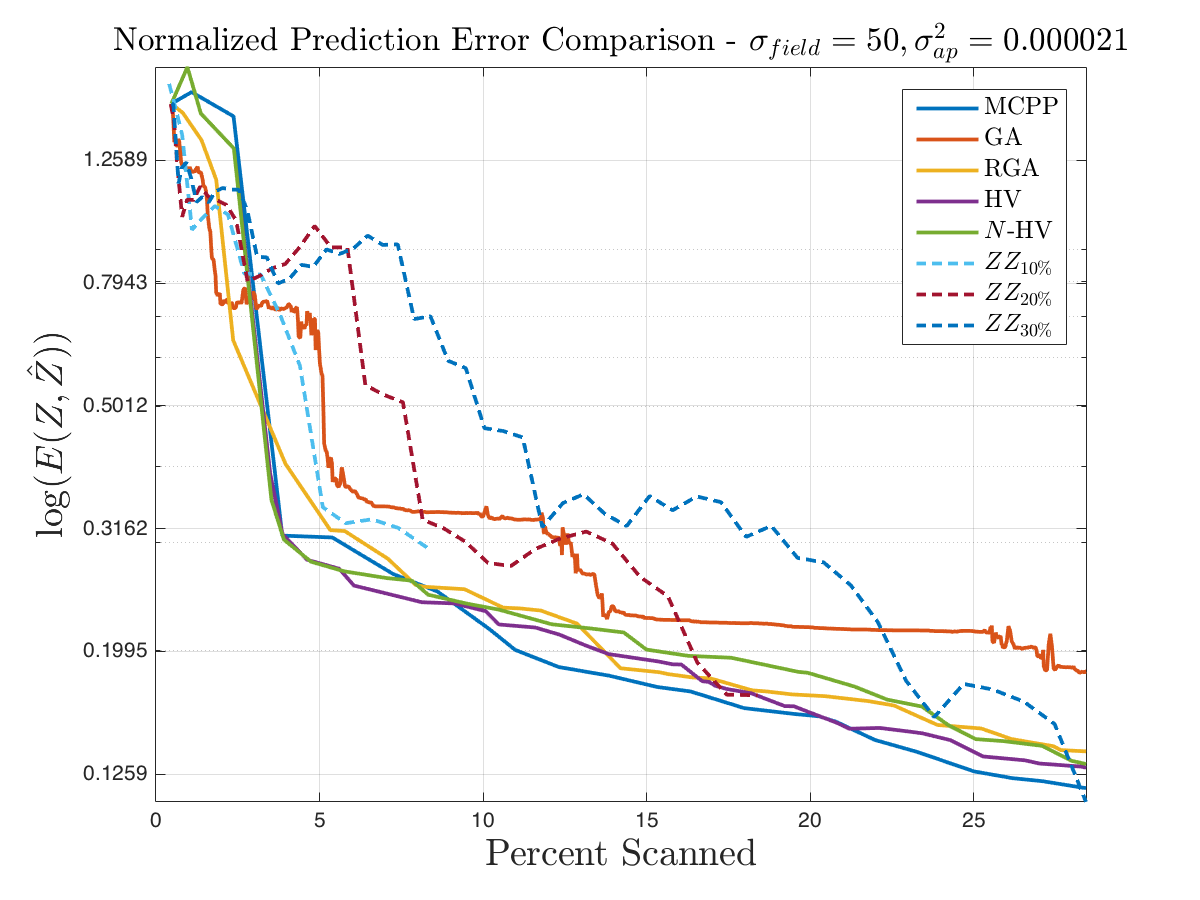
\includegraphics[width=\linewidth]{figures/results/normalized_errors_30p_100x100_sf_50_seed_2_app_50.png}
        \captionsetup{skip=0.20\baselineskip,size=footnotesize}
        \caption{Normalized prediction errors for each method.}
    \end{subfigure}%
    \\
    \begin{subfigure}[t]{0.75\textwidth}
        \centering
        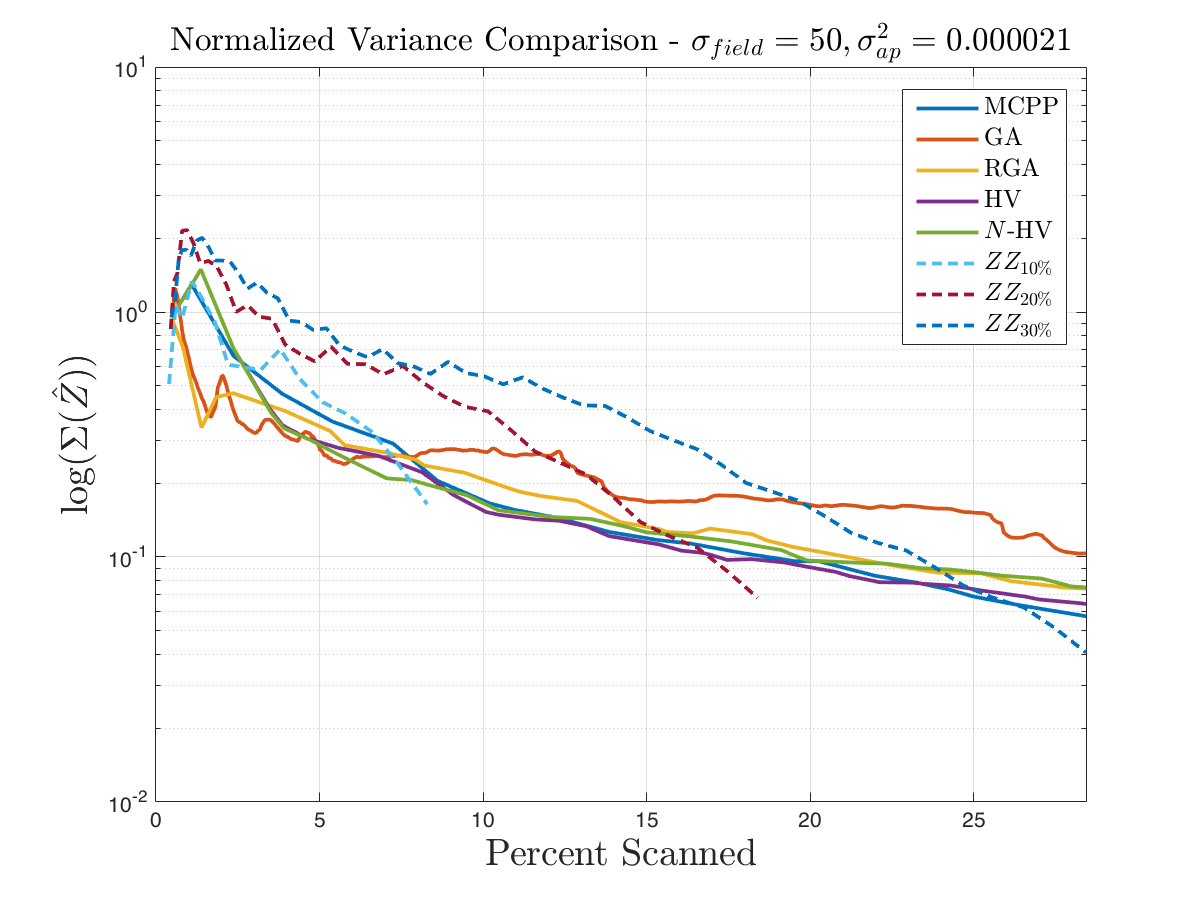
\includegraphics[width=\linewidth]{figures/results/normalized_variances_30p_100x100_sf_50_seed_2_app_50.png}
        \captionsetup{skip=0.20\baselineskip,size=footnotesize}
        \caption{Normalized prediction variances for each method.}
    \end{subfigure}%
    \captionsetup{skip=0.20\baselineskip}
    \caption{Prediction error and variances for an exploration of a field of size $100 \times 100$, $\sigma_{field} = 50$, random seed 2.}
    \label{fig:errvar50}
\end{figure}

\FloatBarrier
\clearpage

\section{Low Spatial Autocorrelation Results}
The methods will be compared on target fields generated with an autocorrelation factor, $\sigma_{field}$, equal to one. A Gaussian filter $G(x,y,1)$ (Equation \ref{eq:gauss_filt}), is convolved with all points on the field.

\begin{figure}[htb!]
    \centering
    \begin{subfigure}[t]{0.3333\textwidth}
        \centering
        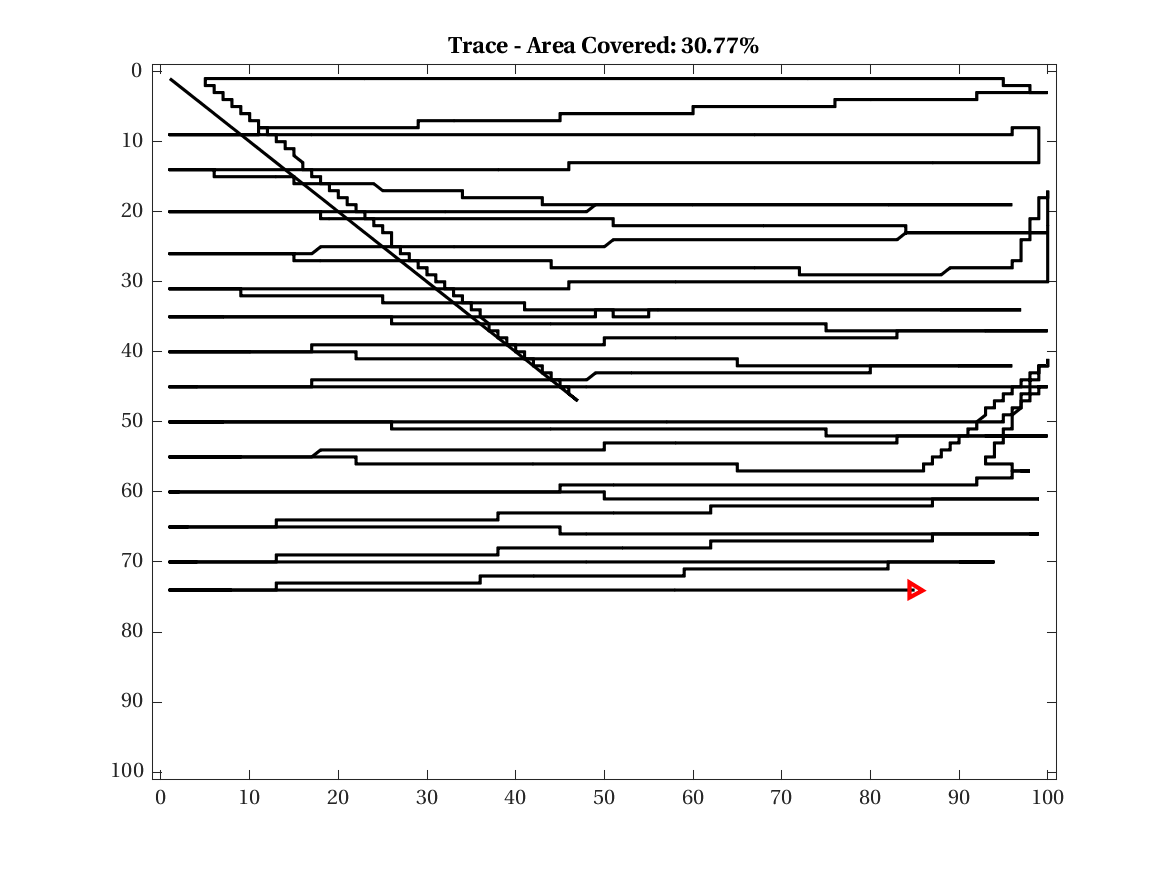
\includegraphics[width=\linewidth]{figures/hbresults/path_nhv_30p_100x100_sf_1_seed_2.png}
        \captionsetup{skip=0.20\baselineskip,size=footnotesize}
        \caption{Highest Variance}
    \end{subfigure}%
    \begin{subfigure}[t]{0.3333\textwidth}
        \centering
        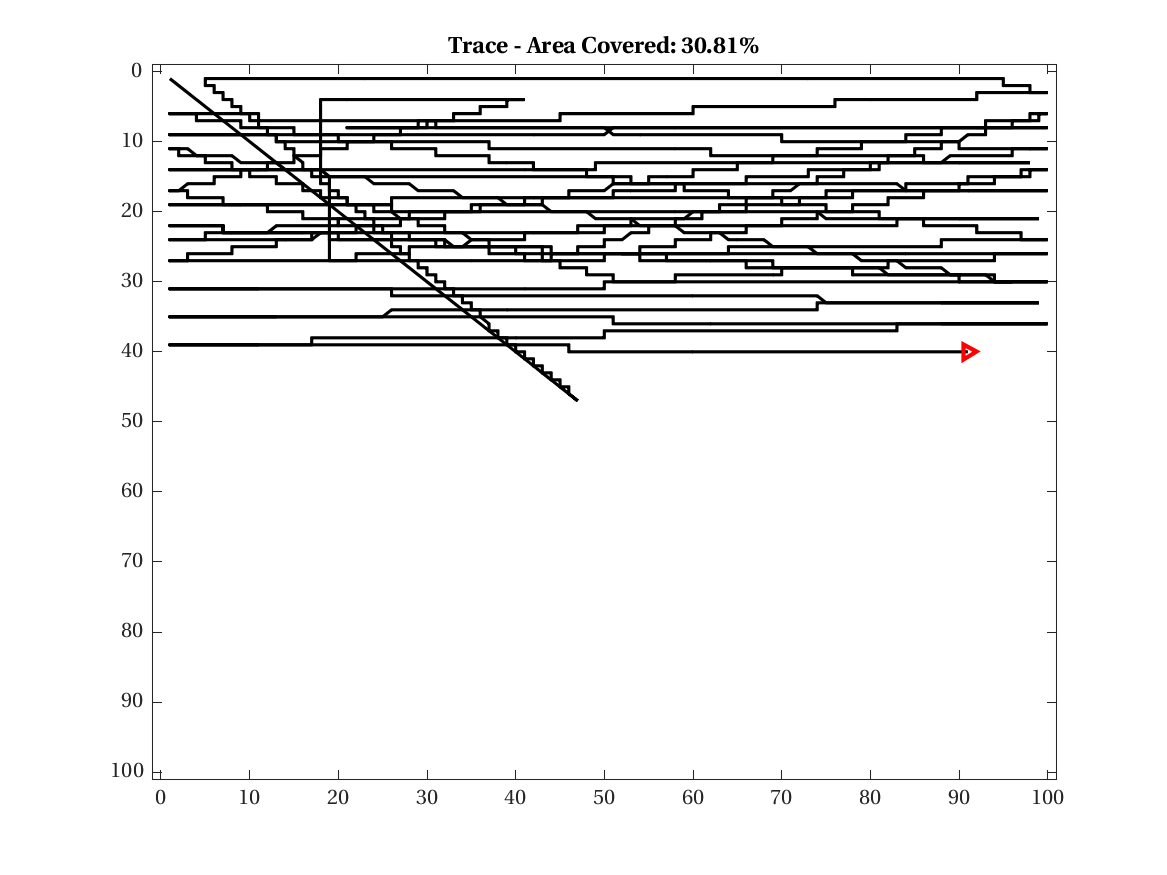
\includegraphics[width=\linewidth]{figures/hbresults/path_nnhv_30p_100x100_sf_1_seed_2.png}
        \captionsetup{skip=0.20\baselineskip,size=footnotesize}
        \caption{$N$ Highest Variance}
    \end{subfigure}%
    \begin{subfigure}[t]{0.3333\textwidth}
        \centering
        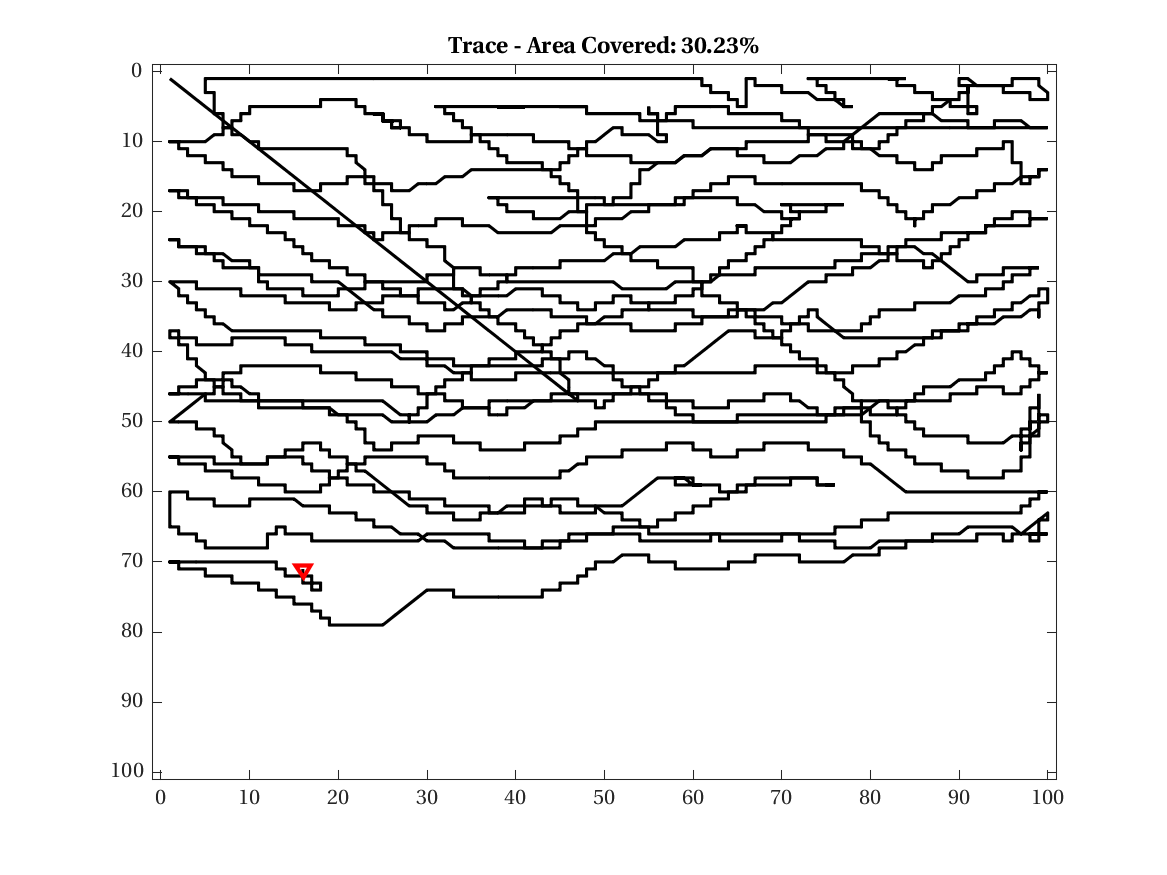
\includegraphics[width=\linewidth]{figures/hbresults/path_mc_30p_100x100_sf_1_seed_2.png}
        \captionsetup{skip=0.20\baselineskip,size=footnotesize}
        \caption{Monte Carlo}
    \end{subfigure}%
    \\
    \begin{subfigure}[t]{0.3333\textwidth}
        \centering
        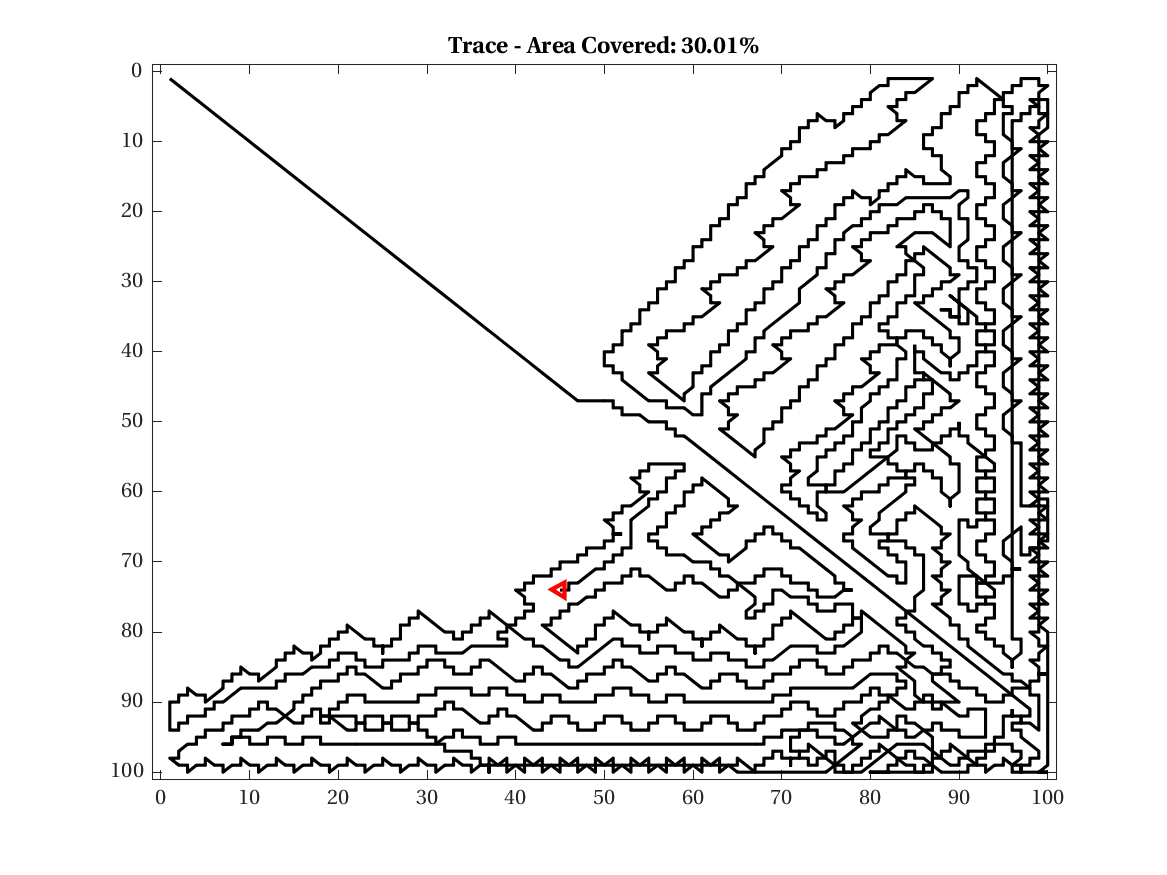
\includegraphics[width=\linewidth]{figures/hbresults/path_gradient_30p_100x100_sf_1_seed_2.png}
        \captionsetup{skip=0.20\baselineskip,size=footnotesize}
        \caption{Gradient Ascent}
    \end{subfigure}%
    \begin{subfigure}[t]{0.3333\textwidth}
        \centering
        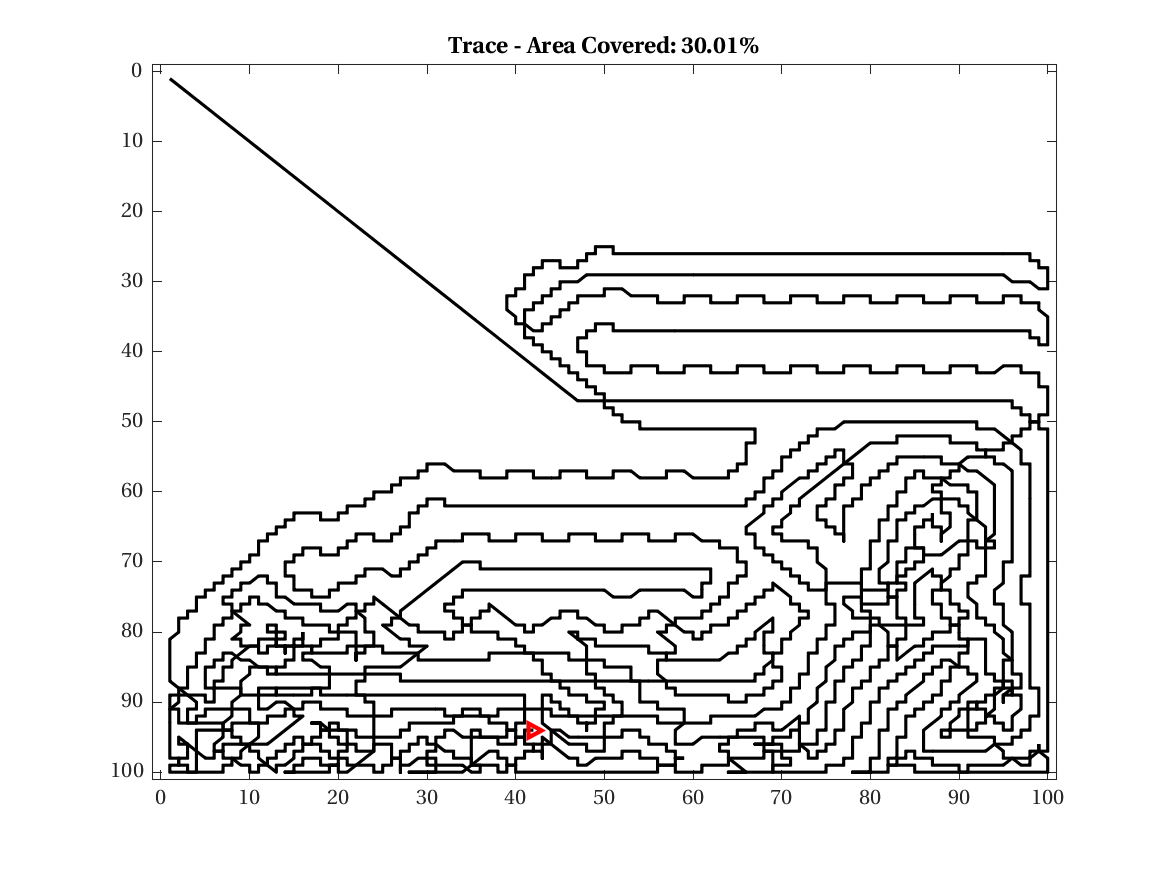
\includegraphics[width=\linewidth]{figures/hbresults/path_gr_30p_100x100_sf_1_seed_2.png}
        \captionsetup{skip=0.20\baselineskip,size=footnotesize}
        \caption{Gradient Range Ascent}
    \end{subfigure}%
    \\
    \begin{subfigure}[t]{0.3333\textwidth}
        \centering
        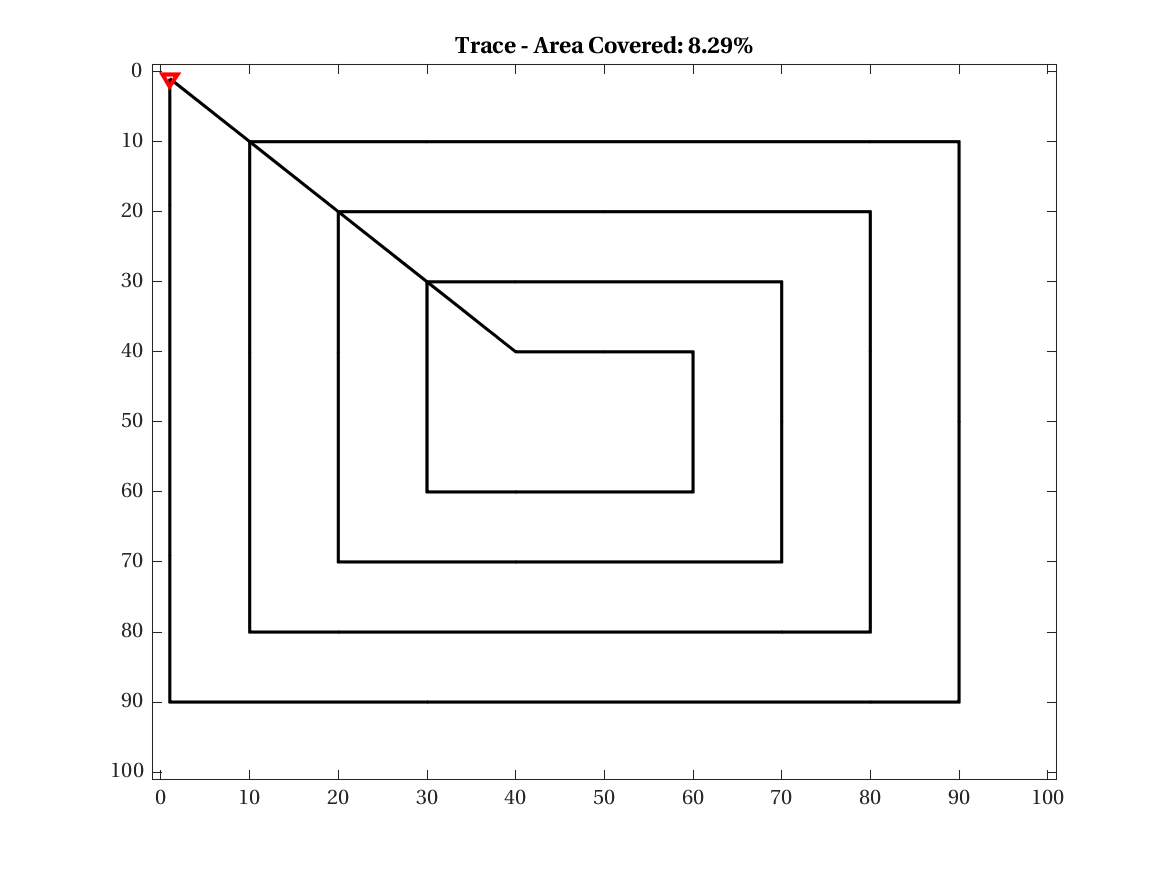
\includegraphics[width=\linewidth]{figures/hbresults/path_zz_10p_100x100_sf_1_seed_2.png}
        \captionsetup{skip=0.20\baselineskip,size=footnotesize}
        \caption{$ZZ_{10}$}
    \end{subfigure}%
    \begin{subfigure}[t]{0.3333\textwidth}
        \centering
        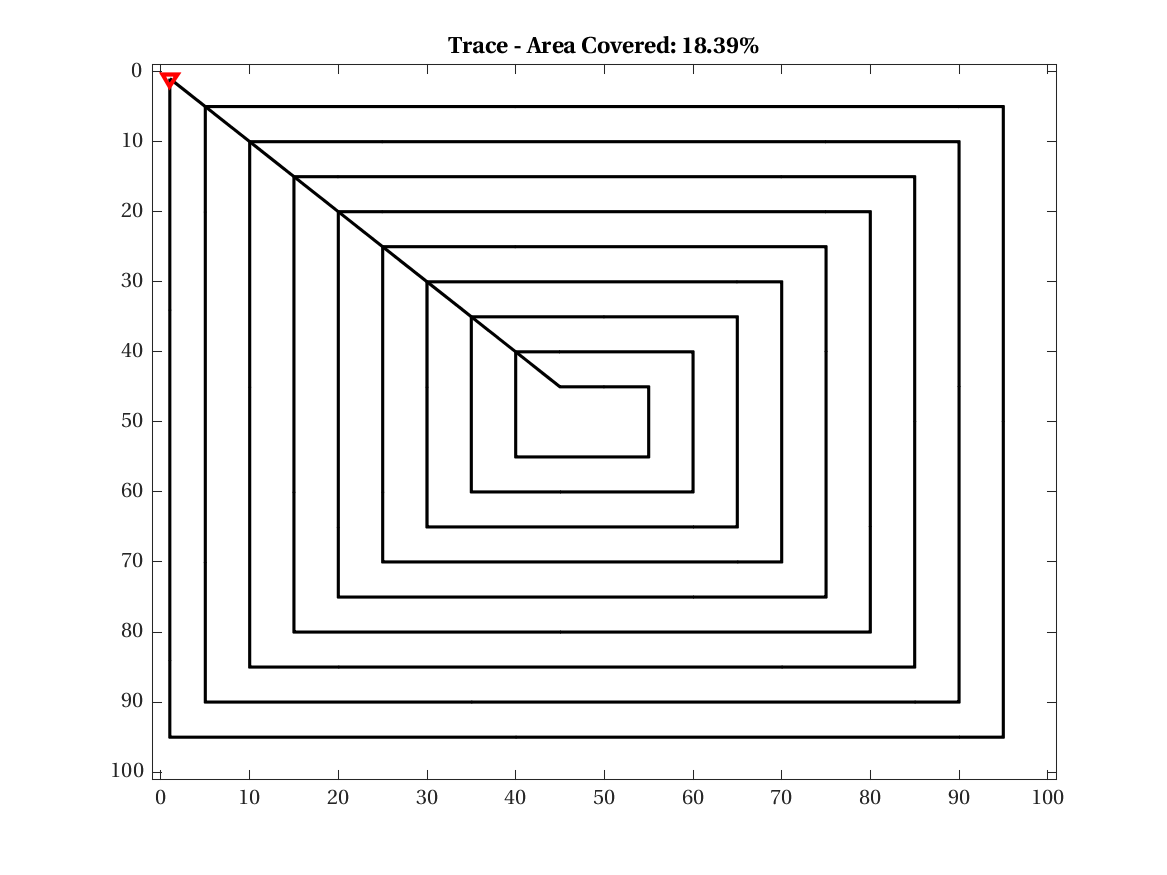
\includegraphics[width=\linewidth]{figures/hbresults/path_zz_20p_100x100_sf_1_seed_2.png}
        \captionsetup{skip=0.20\baselineskip,size=footnotesize}
        \caption{$ZZ_{20}$}
    \end{subfigure}%
    \begin{subfigure}[t]{0.3333\textwidth}
        \centering
        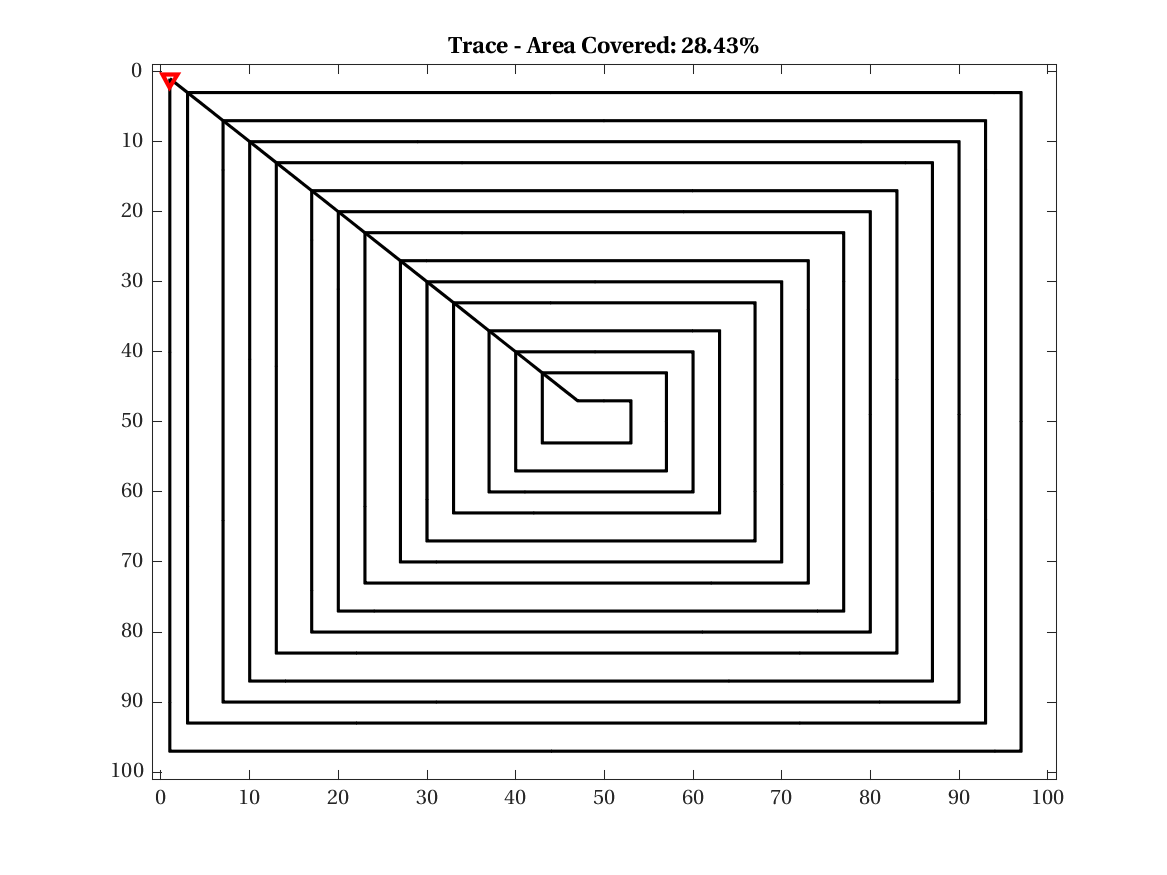
\includegraphics[width=\linewidth]{figures/hbresults/path_zz_30p_100x100_sf_1_seed_2.png}
        \captionsetup{skip=0.20\baselineskip,size=footnotesize}
        \caption{$ZZ_{30}$}
    \end{subfigure}%
    \captionsetup{skip=0.20\baselineskip}
    \caption{Exploration of a field of size $100 \times 100$, $\sigma_{field} = 1$, random seed 2.}
    \label{fig:sf1}
\end{figure}

\begin{figure}[htb!]
    \centering
    \begin{subfigure}[t]{0.75\textwidth}
        \centering
        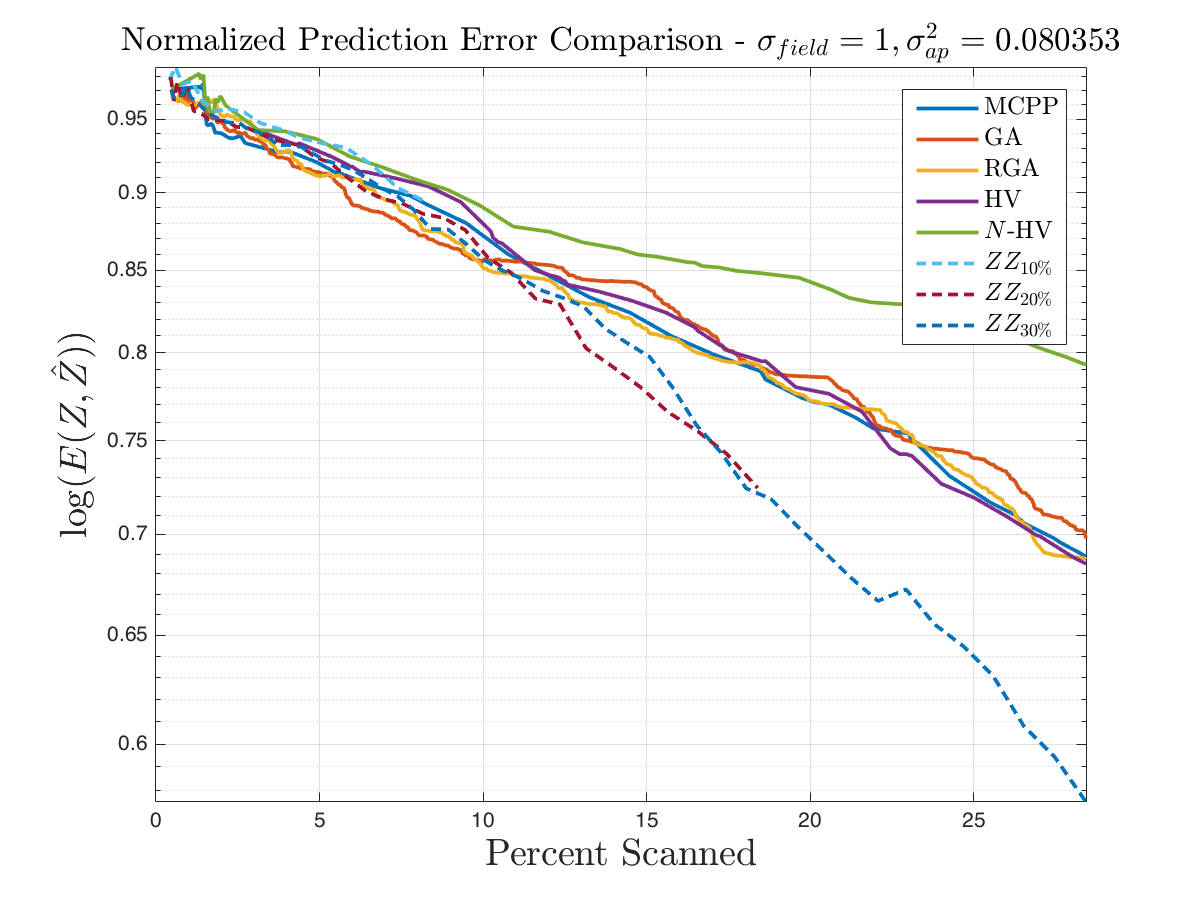
\includegraphics[width=\linewidth]{figures/results/normalized_errors_30p_100x100_sf_1_seed_2_app_50.png}
        \captionsetup{skip=0.20\baselineskip,size=footnotesize}
        \caption{Normalized prediction errors for each method.}
    \end{subfigure}%
    \\
    \begin{subfigure}[t]{0.75\textwidth}
        \centering
        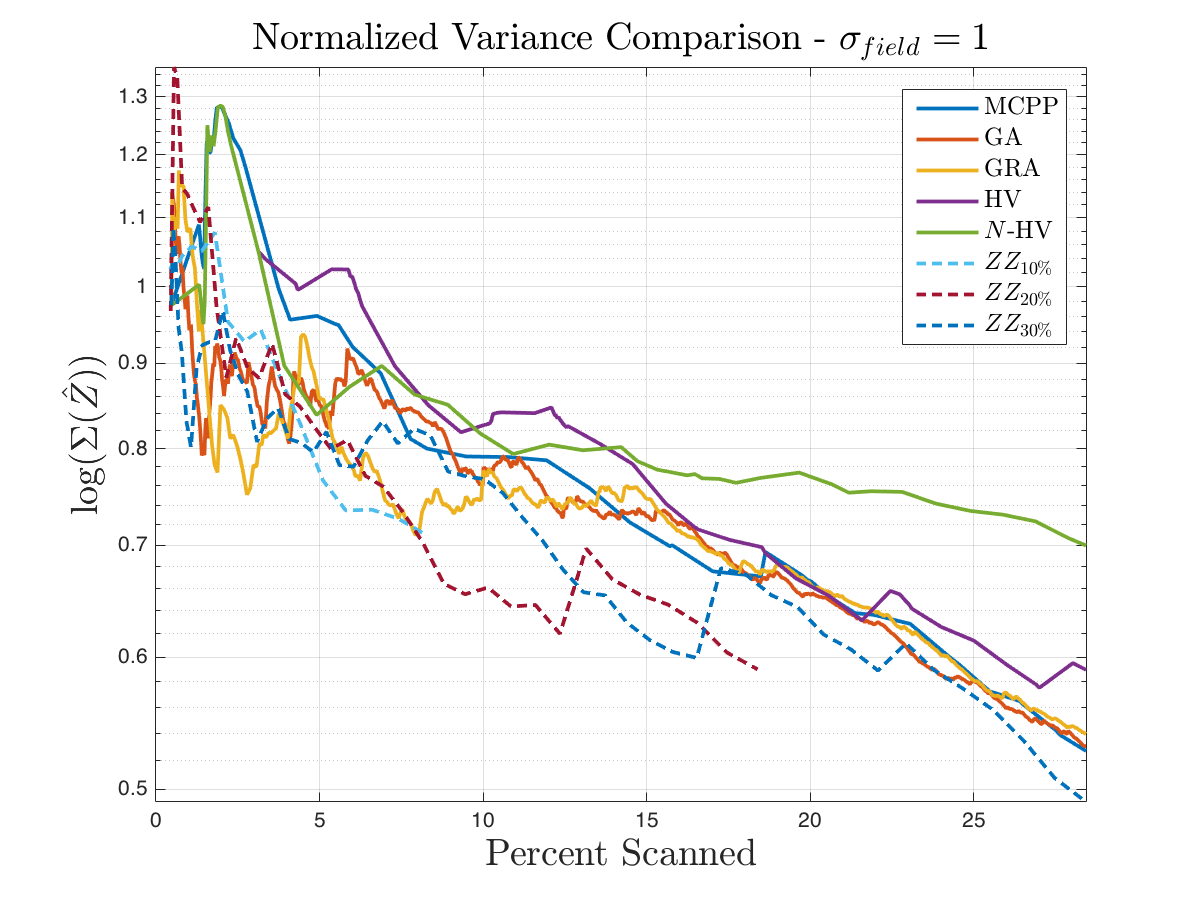
\includegraphics[width=\linewidth]{figures/results/normalized_variances_30p_100x100_sf_1_seed_2_app_50.png}
        \captionsetup{skip=0.20\baselineskip,size=footnotesize}
        \caption{Normalized prediction variances for each method.}
    \end{subfigure}%
    \captionsetup{skip=0.20\baselineskip}
    \caption{Prediction error and variances for an exploration of a field of size $100 \times 100$, $\sigma_{field} = 1$, random seed 2.}
    \label{fig:errvar1}
\end{figure}

\FloatBarrier
\clearpage

% \section{Comparing The Methods}

% \begin{table}[ht!]
% \centering
%   \begin{tabular}{ |p{6cm}||p{1cm}|p{1cm}|p{1cm}|  }
%       \hline
%       \multicolumn{4}{|c|}{Average Final Field Prediction Errors ($\sigma_{field} = 1$)} \\
%       \hline
%       Maximum Percentage Scanned    & 10\% & 20\% & 30\% \\
%       \hline
%       Zig-Zag                       & -- & -- & -- \\
%       Next Highest Value            & -- & -- & -- \\
%       $N$ Next Highest Value        & -- & -- & -- \\
%       Monte Carlo Path Planner      & -- & -- & -- \\
%       \hline
%   \end{tabular}
%   \caption{Comparing field prediction errors for varying coverage limitations on a $100 \times 100$ size field ($\sigma_{field} = 1$). Averaged over two different runs with two random seeds.}
% \end{table}

% \begin{table}[ht!]
% \centering
%   \begin{tabular}{ |p{6cm}||p{1cm}|p{1cm}|p{1cm}|  }
%       \hline
%       \multicolumn{4}{|c|}{Average Final Field Prediction Variances ($\sigma_{field} = 1$)} \\
%       \hline
%       Maximum Percentage Scanned    & 10\% & 20\% & 30\% \\
%       \hline
%       Zig-Zag                       & -- & -- & -- \\
%       Next Highest Value            & -- & -- & -- \\
%       $N$ Next Highest Value        & -- & -- & -- \\
%       Monte Carlo Path Planner      & -- & -- & -- \\
%       \hline
%   \end{tabular}
%   \caption{Comparing field prediction variances for varying coverage limitations on a $100 \times 100$ size field ($\sigma_{field} = 1$). Averaged over two different runs with two random seeds.}
% \end{table}

% \begin{table}[ht!]
% \centering
%   \begin{tabular}{ |p{6cm}||p{1cm}|p{1cm}|p{1cm}|  }
%       \hline
%       \multicolumn{4}{|c|}{Average Final Field Prediction Errors ($\sigma_{field} = 100$)} \\
%       \hline
%       Maximum Percentage Scanned    & 10\% & 20\% & 30\% \\
%       \hline
%       Zig-Zag                       & -- & -- & -- \\
%       Next Highest Value            & -- & -- & -- \\
%       $N$ Next Highest Value        & -- & -- & -- \\
%       Monte Carlo Path Planner      & -- & -- & -- \\
%       \hline
%   \end{tabular}
%   \caption{Comparing field prediction errors for varying coverage limitations on a $100 \times 100$ size field ($\sigma_{field} = 100$). Averaged over two different runs with two random seeds.}
% \end{table}

% \begin{table}[ht!]
% \centering
%   \begin{tabular}{ |p{6cm}||p{1cm}|p{1cm}|p{1cm}|  }
%       \hline
%       \multicolumn{4}{|c|}{Average Final Field Prediction Variances ($\sigma_{field} = 100$)} \\
%       \hline
%       Maximum Percentage Scanned    & 10\% & 20\% & 30\% \\
%       \hline
%       Zig-Zag                       & -- & -- & -- \\
%       Next Highest Value            & -- & -- & -- \\
%       $N$ Next Highest Value        & -- & -- & -- \\
%       Monte Carlo Path Planner      & -- & -- & -- \\
%       \hline
%   \end{tabular}
%   \caption{Comparing field prediction variances for varying coverage limitations on a $100 \times 100$ size field ($\sigma_{field} = 100$). Averaged over two different runs with two random seeds.}
% \end{table}
